\documentclass[a4paper,12pt,twoside,openright]{report}

\usepackage[utf8]{inputenc}
\usepackage[T1]{fontenc}
\usepackage[hidelinks]{hyperref}
\usepackage[backend=biber]{biblatex}
\usepackage[english]{babel}
\usepackage{color}
\usepackage{graphicx}
\usepackage{import}
\usepackage{csquotes}
\usepackage{geometry}
\usepackage{listings}

% ------------------------ Custom listings

\renewcommand{\ttdefault}{pcr}
\usepackage{styling/javascript-listing}
\usepackage{styling/rust-listing}
\usepackage{styling/wasm-listing}
\usepackage{styling/yaml-listing}
\usepackage{styling/generic-code-listing}

% ------------------------ Page styling

\usepackage{styling/page}

% ------------------------ Custom hypthenations
\hyphenation{Web-As-sem-bly}

% ------------------------ Graphics
\graphicspath{{./images/}}

% ------------------------ Bibliography
\addbibresource{bibliography.bib}

% ------------------------ Actual document
\begin{document}
  \begin{titlepage}
  \begin{center}
    \large
    UNIVERSITÀ DEGLI STUDI DI BERGAMO \\
    \vspace{0.5cm}
    \normalsize
    Dipartimento di Ingegneria Gestionale, dell'Informazione e della Produzione \\
    Corso di Laurea Magistrale in Ingegneria Informatica \\
    Classe LM-32

    \vspace*{3cm}

    \Huge
    \textbf{Thesis title}

    \vspace{0.5cm}
    \LARGE
    Thesis Subtitle
  \end{center}

  \vfill

  \begin{flushleft}
    Relatore \\
    Chiar.mo Prof.\ Paraboschi Stefano
  \end{flushleft}

  \vspace{1cm}

  \begin{flushright}
    Tesi di Laurea Magistrale \\
    Michele BERETTA \\
    Matricola n.\ 1054365
  \end{flushright}

  \vfill

  \begin{center}
    ANNO ACCADEMICO 2021/2022
  \end{center}
\end{titlepage}
  \emptypage
  \begin{abstract}
Nowadays, web applications' needs are more sophisticated and demanding than in the past.
Efficiency and security are hence important points that must be addressed. However JavaScript,
the de facto standard of scripting languages on the web, is not able to meet these requirements.

In order to compensate for JavaScript's downsides, \textit{WebAssembly} (WASM) was introduced.
WASM is a new language that is ``designed for efficient execution and compact representation of code
on modern processors including in a web browser'' \cite{wasm-w3c-announcement}, and strives to
improve both performance and power consumption.
Although WASM was conceived to run in browsers, it can also be run directly on the host with the aid of runtimes, such as
\textit{Wasmtime} and \textit{Wasmer}, that do provide a fair level of security.
In some use cases, however, the provided security level is not enough and solutions to enhance it
are necessary.

The aim of this thesis work is to explore how these runtimes can be further restricted
through the aid of Linux Security Modules so to improve security and give more control to the user.
\end{abstract}
  \emptypage
  \toc
  \emptypage

  \clearpage
  \pagenumbering{arabic}
  
  \chapter{Introduction}
  \section{The Web}

\subsection{Basic structure}

The \textit{World Wide Web}, or more commonly \textit{Web}, is a collection of documents and other resources
that can be shared among various devices via the \textit{Internet}.

The resources shared are usually in the form of \textit{web pages}, documents whose structure is defined with HTML
(\textit{Hypertext Markup Language}) and whose styles are declared with CSS (\textit{Cascade Style Sheet}).
Other kind of resources include anything ranging from images, videos, audio, software, and source code.

However, web pages are \textit{static} if they only use HTML and CSS, and cannot do much aside from showing content. A programming
language is hence needed to make the web \textit{dynamic}. Among all technologies and languages, nowadays
only JavaScript survives as the de facto standard language, used for both simple scripts and complex applications.

\subsection{JavaScript}
\label{sec:introduction-javascript}

\textit{JavaScript}, or \textit{JS} when abbreviated, is a high-level, dynamic, weakly typed programming language
that together with HTML and CSS is at the core of the World Wide Web. It conforms to the ECMAScript standard \cite{ecma-262}
and it can be both interpreted and \textit{just-in-time compiled}.
A notable language which is a superset of JavaScript is \textit{TypeScript}, developed by Microsoft, that
introduces static typing and can be transpiled to JavaScript.

\begin{code}[language=javascript, caption=A simple example of JavaScript]
function fact(n) {
  if (n == 0) return 1;
  return n * fact(n - 1);
}

function showFactorial() {
  let div = document.getElementById('output');
  let input = document.getElementById('number');
  let n = parseInt(input.text);

  if (n < 0) {
    div.innerHTML = 'Not defined';
  } else {
    div.innerHTML = fact(n);
  }
}

document
  .getElementById('get-factorial')
  .addEventListener('click', showFactorial)
\end{code}

However, JavaScript is ill-equipped when it comes to performance-critical modern web
pages - from this needs were born technologies such as \textit{asm.js}, \textit{Native Client}, and eventually \textit{WebAssembly}.
The main downsides of JavaScript that brought the need for WebAssembly are:
\begin{itemize}
  \item JavaScript is \textit{always} represented as a text format, so it must be parsed by the user's browser for it to be compiled and enhanced;
  \item JavaScript is dynamically typed, hence optimisations for JS (when possible) have to occur
        in the browser, when all JS files have been received;
        for example, JS has only two numeric type (a double-precision IEEE 754 value and a \textit{BigInt}
        for numbers bigger than $2^{53}$) and this restricts the usable CPU instructions;
  \item JavaScript has a number of security vulnerabilities that WebAssembly strives to eliminate by design;
        a common security vulnerability\footnote{Software vulnerabilities are the most common, but hardware vulnerabilities have also been found \cite{spectre}.}
        in the JavaScript world is \textit{cross-site scripting} (XSS), which is a violation of the
        same-origin policy and occurs when an attacker is able to inject a malicious script in a target website;
        another vulnerability is \textit{cross-site request forgery} (CSRF), in which malicious code on an attacker's website
        tricks the user's browser, so that it takes actions not desired by the user.
\end{itemize}

\subsection{Web browsers and JavaScript runtimes}

A \textit{web browser} is a piece of software for accessing web pages shared on the World Wide Web, or a
local website. Browsers natively support the rendering of HTML and CSS, and feature an engine able to run JavaScript or, more commonly,
to just-in-time compile it in order to improve performance.

Browsers can also mitigate the risk provided by the common JavaScript vulnerabilities mentioned in Section \ref{sec:introduction-javascript}
by using two main methods - \textit{sandboxing}, so that JS isn't allowed to perform general-purpose
programming tasks like working directly with files\footnote{Although, there are APIs that can grant access to a ``virtual drive''
only when explicitly allowed by the user \cite{filesystem-mdn}, so access to the user's file system is not possible.},
and \textit{same-origin policy} constraints, in which scripts from one website have access to data from the same website but not from others.

JavaScript can not only be executed on a browser, but also on so called ``back-end''
runtimes\footnote{Opposed to ``front-end'', which usually pertains to the browser.}.
These runtimes offer custom libraries that permit JavaScript to access the file system, to make network requests,
spawn child processes and build complex applications, for example web servers.
Two notable open-source runtimes are \textit{Node.js}\footnote{\url{https://nodejs.org/}} and \textit{Deno}\footnote{\url{https://deno.land}},
both built on top of Google's V8 engine.
The first is older, initially released in 2009, and has a package manager called \textit{npm}
in order to manage its vast ecosystem of JS packages.
Deno, on the other hand, is a more modern runtime written in Rust, includes support for TypeScript out of the box
and is \textit{secure by default} since it blocks all file, network, and environment access unless explicitly enabled.

\section{WebAssembly}

\subsection{Description and motivations}

\textit{WebAssembly} \cite{wasm-website} is a binary instruction format for a stack-based virtual machine.
It is designed to be a portable compilation target, so that different languages can be deployed on the web.
It was announced in 2015 and implemented by major browsers by 2017, and as of May 2022 is supported
by 93\% of all browsers \cite{caniuse, webassembly-mdn}.
WebAssembly main goals are the following \cite{bringing-the-web-up-to-speed-2017}:
\begin{itemize}
  \item \textit{security}, since code on the Web originates from untrusted sources;
  \item \textit{speed}, by using ahead-of-time optimisations in a similar manner as native machine code;
  \item \textit{portability}, since the web spans many devices, architectures, operating systems, and browsers;
  \item and finally \textit{compactness}, because code is transmitted over the network and must reduce load times as much as possible.
\end{itemize}

There were previous attempt at solving the problem of having safe, fast, and portable low-level code on the Web,
such as \textit{ActiveX}, \textit{Native Client}, and \textit{asm.js}.

\textit{ActiveX} \cite{activex} was a Microsoft's technology for code-signing x86 binaries to run on the web, and relied only
on this signing. Hence, it achieved security through a trust model instead of technical construction.
\textit{Native Client} \cite{native-client} introduced the first sandboxing technique for x86, ARM or MIPS machine code,
which was statically validated. Lastly, \textit{asm.js} \cite{asmjs} is a specialised subset of JavaScript, which is one of the target
languages of \textit{Emscripten} \cite{emscripten}, a compiler toolchain able to compile C/C++ applications in order to have them
run on browsers or on other JavaScript runtimes.

WebAssembly is available as a target for various languages, such as C/C++ with the aid of Emscripten, Rust,
AssemblyScript\footnote{A language with a syntax similar to TypeScript.}, Go, Kotlin, Swift, and Zig.
The compiled binary can be then used from JavaScript on the web, or with Node.js or Deno, or even as a CLI application
with the aid of \textit{WebAssembly runtimes} and the \textit{WebAssembly System Interface}
for accessing system resources (see Section \ref*{sec:introduction-wasi}).

WebAssembly resolves many of the problems of JavaScript, the major ones being:
\begin{itemize}
  \item being represented with a \textit{binary} format, parsing on the client is faster and simpler;
  \item having a static type systems, optimisations can be done earlier at compile time, and not on the browser once all the files
        have already been transferred;
\end{itemize}

\subsection{Overview of the language}

Although WebAssembly is a binary code format, it can also be written with \textit{S-expressions}
in order to be more readable.
Each binary takes the form of a \textit{module}, which contains \textit{functions}, \textit{global} variables,
\textit{tables}, and \textit{memories}. Each of these can be exported to be used in the embedder, and a module can also import functionalities.
While a module is a static representation of a program, an \textit{instance} is the dynamic one.
A module can be instantiated by the embedder (e.g., a JavaScript virtual machine).

\begin{code}[language=wasm, caption={Recursive factorial written in WebAssembly S-expressions}, label=lst:wasm-fact]
  (module
    (func $fact (param $x i64) (result i64)
      (if (result i64) (i64.eqz (local.get $x))
        (then (i64.const 1))
        (else
          (i64.mul
            (local.get $x)
            (call $fact
              (i64.sub (local.get $x) (i64.const 1)))))))
    (export "fact" (func $fact)))
\end{code}

WebAssembly is a typed language, but there are only four basic \textit{value types} - integers and IEEE 754 floating
point numbers, each in 32 and 64 bit variants. There are no distinction between signed and unsigned integers,
but instructions that depends on the present of the sign are marked with an explicit suffix.

\textit{Functions} are typed, take a sequence of values as a parameter, and returns another sequence of values.
They cannot be nested inside each other. The content of the call stack for execution are separate from the data
portion of the memory, and cannot be accessed directly by WebAssembly.
The code inside a function consists of a series of \textit{instructions} that modify an implicit operand stack,
either by declaring local variables or applying operations to the value already on the stack.
Functions can be called either \textit{directly} by using an index that identifies a function, or \textit{indirectly},
i.e., dynamically through a global \textit{table}. In this second case, only the function's type signature is validated.

WebAssembly has also support for \textit{traps} - in a similar manner to an exception, a trap aborts the current
computation, and control is given back to the embedder. For example, when embedded in JavaScript, a trap will
throw a JavaScript exception.

The main memory layout that WebAssembly uses is a \textit{linear memory} (or simply \textit{memory}) represented
by an array of bytes. A \textit{linear memory} is a simple addressing technique in which memory appears to the
program as a single contiguous access space \cite{processor-microarchitecture}, which the CPU can access both directly as well as linearly
without resorting to memory segmentation or pagination schemes, enhancing flexibility and reducing latency.
Each module can define no more than one memory, which can grow by one or more
\textit{pages}\footnote{A page is 64 KiB large.} if the need arises.
Access to the individual locations is done through addresses, represented as unsigned integers,
which are dynamically checked against memory size\footnote{On 64 bit platforms the WebAssembly engine
can make use of virtual memory techniques to eliminate this checks, see \cite{bringing-the-web-up-to-speed-2017}}
(out of bounds accesses result in a trap).
Linear memory also brings security benefits - it is disjoint from the code space, the execution stack and the engine's
data structures \cite{bringing-the-web-up-to-speed-2017}; hence, compiled program cannot corrupt directly their own execution
environment or perform undefined behaviour.

Lastly, WebAssembly doesn't provide arbitrary jumps but \textit{structured control flow},
so that the code can be validated in a single pass and prevent common control flow attacks.

\subsection{Problems with WebAssembly}

Since languages with manual memory management, such as C/C++, can be compiled into WebAssembly,
it is natural to ponder how memory vulnerabilities affect WebAssembly binaries.
In the original paper it is mentioned that ``a buggy or exploited WebAssembly program can make a mess of the data in its own memory''
\cite{bringing-the-web-up-to-speed-2017}, in light of the fact that the call stack is not accessible by the program.

However, even though WebAssembly strives for security, binaries can be still exploited with both traditional attacks,
such as buffer overflows, and attacks that aren't applicable in traditional native binaries, e.g., overwriting
string literals in memory \cite{binary-security-wasm-2020}.

The paper shows that it is possible to obtain a write primitive given a WebAssembly binary compiled from vulnerable C/C++ code,
by means of stack-based buffer overflows and heap metadata corruption, and it is possible to overwrite stack, heap, and ``constant''
data, since the linear memory does not have a read-only section. It would be possible then, for example, to overwrite the name
of a file that was encoded as a string literal in the original program.

Another problem shown in the same paper is the redirection of indirect calls. Since WebAssembly allows indirect calls
to functions through a function table, an attacker could divert the execution by overwriting an integer in linear memory
that serves as an index into the table section. WebAssembly limits this ability with two mechanisms - not all functions
may appear in the table, but only those that can be indirectly called, and all functions call are type checked.
So, redirecting indirect calls is possible only within the class of functions with the same type.

Lastly, it is possible to enable remote code execution when including vulnerable WebAssembly in an application.
This is because functions that have different types in one language can be mapped onto functions with the same type
in WebAssembly. For example, a log function that in C has the signature \texttt{void log(int)}, and a function such as
\texttt{void exec(const char* cmd)} both become functions with only one \texttt{i32} param in WebAssembly.
This enables the indirect diversion described in the previous paragraph if the two functions can be indirectly called.

\subsection{WASI - WebAssembly System Interface}
\label{sec:introduction-wasi}

The \textit{WebAssembly System Interface} (WASI) \cite{wasi} is a modular system interface for WebAssembly.
It focuses on security and portability so that WebAssembly binaries can be targeted by different languages
and then be safely run on different platforms.
Its API provides access to several OS-like features, such as file systems and Berkeley sockets.
The two languages that have good interoperability at the moment are Rust, where the compiler directly supports targeting both WASM and WASI,
and C/C++, either through Emscripten or a custom prebuilt \textit{Clang} toolchain\footnote{\url{https://github.com/WebAssembly/wasi-sdk}}.

A binary that uses WASI can be run using a CLI runtime, such as \textit{Wasmtime} \cite{wasmtime} or \textit{Wasmer} \cite{wasmer},
or using a browser polyfill (an example is visible in \cite{wasi-polyfill}).
The approach taken for the sandboxing by these runtimes is based on a \textit{capability-based security model} \cite{wasmtime-security-sandboxing},
so that access to the file system and other resources must be explicitly given. Capabilities can be either \textit{static}, which
are represented by the list of imports of the WebAssembly module to run, or \textit{dynamic}, i.e., specific flags
specified with custom command-line arguments at execution time.
Moreover, when given permissions to write to a terminal, a program could print characters recognised as control
sequences that may have side effects and confuse or misled user (a harmless example is clearing the screen).
Hence, all writes to output streams are filtered in order to prevent this type of behaviour.

CLI runtimes have some particular features and properties:
\begin{itemize}
  \item it is possible to \textit{sandbox} entire directories by \textit{preopening} them, and eventually mapping them to custom paths,
        in order to have the file descriptors available; it is not possible to escape this sandbox using the parent directory \texttt{..}
        or soft links, but it is possible to escape using hard links;
        this is because hard links point directly to the \textit{data} on disk, and behave as a full fledged copy of the linked file, while soft links
        only point to an existing \textit{file} - this is why using hard links is possible to ``escape'' sandbox;
  \item the \textit{directory} is the finest granularity available to the preopen action - once access is given to a specific directory, all files and subdirectories are
        visible, and it is not possible to restrict permissions (all files are readable and
        writable) when using the command line runtime wrapper\footnote{It is possible to specify a basic set of permissions when using the WASI runtime library in another language, such as in Rust,
        see example at \url{https://docs.rs/wasmer-wasi/latest/wasmer_wasi/struct.WasiState.html}.};
  \item when using C, the WebAssembly binary can create files with specific user permissions on Linux, e.g., executable files;
  \item when listing files in a directory, the only files that are visible are the ones that were already present at the preopening of the directory,
        but files added after the preopen can be ``seen'' if their name is known (i.e., they can be opened, read or written in accordance with given permissions);
  \item any change made to a file by any process is reflected in what the compiled WebAssembly binary is able to read;
  \item environment variables are not accessible by default, but they must be explicitly declared and given access to;
  \item the WebAssembly memory is effectively sandboxed - the compiled program cannot access memory outside its sandbox, otherwise a trap is raised;
  \item not all ``classic'' functionality is available - when compiling C with the custom prebuilt toolchain,
        functions such as \texttt{system}, \texttt{execv}, and \texttt{fexecve} are not available,
        so it is not possible to execute arbitrary commands or files;
  \item fileless execution isn't feasible, since \texttt{memfd\_create} is not available due to the missing
        \texttt{sys/mman.h}\footnote{This library can be emulated, but \texttt{memfd\_create} is still not available.}.
\end{itemize}

By using the \textit{wasm2c} tool available in the \textit{WebAssembly Binary Toolkit}\footnote{\url{https://github.com/WebAssembly/wabt}},
C code can be compiled into WebAssembly and then converted back to C.
This way, a traditional C program can use directly the functions made available from the original C library with an added sandbox
that allows code isolation. The sandboxed library cannot access locations outside its allocated memory without causing a trap,
halting the execution, and giving back control to the embedder.
Similarly, the user C code cannot access the sandboxed memory directly, and, if the code were to attempt to do so,
it would result in a segmentation fault.

Lastly, as highlighted in \cite{wasmtime-security-sandboxing}, Spectre mitigations are not yet implemented, but are a topic of
ongoing research.

\subsection{WebAssembly as a fault isolation tool}

Since WebAssembly is \textit{sandboxed}, it is possible to isolate libraries that could be a frequent source of
vulnerabilities by compiling them to WebAssembly before their use.

An example is shown with the \textit{RLBox} project \cite{wasm-firefox-isolation-2020, rlbox-docs},
a framework that supports efficient sandboxing with modest performance overhead,
that has been integrated into Firefox in order to sandbox the \texttt{libGraphite} font shaping library.
RLBox ensures that whatever library is sandboxed is also memory isolated from the rest of the application,
and all these boundary crossings are explicit. The isolation is enforced by sandboxing mechanisms, such as
WebAssembly \cite{wasm-sandboxing-firefox}, and to ensure that application code doesn't use unsafe values
originated in the sandbox, RLBox differentiates between \textit{tainted} and \textit{untainted} values
through the use of the C++ type system.

Even the WASI interface is able to segregate a WebAssembly binary, since it is effectively \textit{sandboxed}
- all interactions with the embedding environment must be done through explicit exports and imports, and the memory is
bound checked at runtime. Hence, the WebAssembly program cannot access data outside its assigned memory, and the
embedder cannot access memory assigned to the WebAssembly code directly.

\section{Linux Security Modules}

The \textit{Linux Security Modules} (LSM) \cite{lsm-2002, kernel-lsm}
is a lightweight, general purpose, access control framework for the Linux Kernel.
It provides a mechanism for various security checks to be hooked by kernel extensions.
These extensions are not loadable kernel modules, but they can either be chosen at
compile-time via specific flags, such as \texttt{CONFIG\_DEFAULT\_SECURITY}, or overridden at boot-time.

The LSM is used primarily by \textit{Mandatory Access Control} (MAC) extensions to
provide a security policy. However, other extensions can be built with the LSM framework
in order to implement specific changes when they cannot be obtained with the functionality Linux itself.

Some projects that use LSM include:
\begin{itemize}
  \item \textit{SELinux} \cite{selinux}, i.e., \textit{Security Enhanced Linux}, that provides a mechanism for supporting advanced and fine-grained access control policies, as well as MAC;
  \item \textit{Smack} \cite{smack}, a kernel based implementation of MAC with simplicity as one of its primary goals;
  \item \textit{AppArmor} \cite{apparmor}, a MAC style security extension that implements a task centred policy.
\end{itemize}

\begin{figure}[ht]
  \centering
  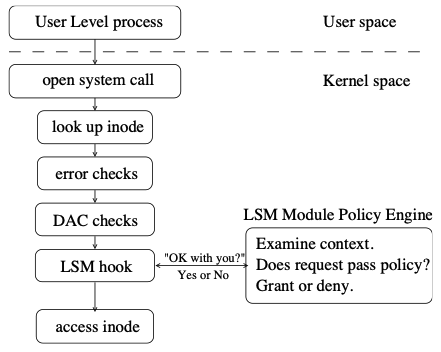
\includegraphics[width=0.6\linewidth]{lsm-hook-architecture.png}
  \caption{LSM Hook Architecture, from \cite{lsm-2002}}
  \label{fig:lsm-hook-architecture}
\end{figure}

\subsection{Landlock}
\label{sec:intro-lsm-landlock}

\textit{Landlock} \cite{landlock-kernel, landlock-user-space} is a security feature available since Linux 5.13
that uses the LSM framework in order to provide scoped access control
so that any process, even when unprivileged, can securely restrict itself.
This can help mitigate the security impact of bugs or unexpected/malicious behaviour
in user space applications.

Landlock employs the concept of \textit{rule}, which describes an action
on an object. An object is (currently) a file hierarchy, and actions are
defined with access rights, such as executing, reading or writing files, making
symbolic links and so on.
A set of rules is called a \textit{ruleset}, and it can restrict both the thread
using it and its future children, created either by spawning a new thread, as well
as using the \textit{fork} system call.

Notably, Landlock does not permit the definition of exceptions.
For example, let us suppose we have a directory \texttt{dir1}, which contains two files
\texttt{file1} and \texttt{file2}. We can define a ruleset that allows
reading and writing files for \texttt{dir1}.
However, if we then define another ruleset comprising only of read operations
for \texttt{file1}, the permissions specified for \texttt{dir1} are still
valid, so when a process restricts itself it is still able to write to \texttt{file1}.

Other limitations of Landlock include the impossibility for a thread to modify its own topology
(e.g., via \textit{mount}), a limit of 16 layers of stacked rulesets and the impossibility to
restrict special file systems, such as kernel file systems (e.g., nsfs).

In case of multiple consecutive self-restrictions, the result is the intersection
of all rulesets - if a process first restricts itself allowing all read and writing operations,
and then restricts itself again with only reading permissions, the result is equivalent
to a single restriction made with a ruleset that permits only reading operations.

Landlock can be used directly when writing C/C++ code in Linux with the
\texttt{<linux/landlock.h>}\footnote{Examples of code available at \cite{landlock-user-space}.}
header, or by using libraries that provide these bindings to other languages,
such as \texttt{go-landlock} \cite{go-landlock}
for Go and \texttt{rust-landlock} \cite{rust-landlock} for Rust.

Landlock employs a series of flags to restrict a sandboxed process to a set of actions on files and
directories opened after the sandboxing operation (those opened before are not affected).
As highlighted in \cite{landlock-user-space}, the file system flags for files are:
\begin{itemize}
  \item \texttt{LANDLOCK\_ACCESS\_FS\_EXECUTE}, to execute a file;
  \item \texttt{LANDLOCK\_ACCESS\_FS\_WRITE\_FILE}, to open a file with write access;
  \item \texttt{LANDLOCK\_ACCESS\_FS\_READ\_FILE}, to open a file with read access.
\end{itemize}

Directories can receive a wider range of access rights, including the previous ones and the following ones.
All of them, except the first, are applied to the content of a directory and not to the directory
itself\footnote{This means that, for example, if \texttt{LANDLOCK\_ACCESS\_FS\_REMOVE\_DIR} is given to a directory $d$, it
allows the removal of empty directories \textit{inside} of $d$, and not of $d$ itself.}.
\begin{itemize}
  \item \texttt{LANDLOCK\_ACCESS\_FS\_READ\_DIR}, to open a directory or list its content\footnote{Applies to subdirectories as well.};
  \item \texttt{LANDLOCK\_ACCESS\_FS\_REMOVE\_DIR}, to remove an empty directory or rename one;
  \item \texttt{LANDLOCK\_ACCESS\_FS\_REMOVE\_FILE}, to unlink or rename a file;
  \item \texttt{LANDLOCK\_ACCESS\_FS\_MAKE\_CHAR}, to create, rename or link a character device;
  \item \texttt{LANDLOCK\_ACCESS\_FS\_MAKE\_DIR}, to create or rename a directory;
  \item \texttt{LANDLOCK\_ACCESS\_FS\_MAKE\_REG}, to create, rename or link a regular file;
  \item \texttt{LANDLOCK\_ACCESS\_FS\_MAKE\_SOCK}, to create, rename or link a socket;
  \item \texttt{LANDLOCK\_ACCESS\_FS\_MAKE\_FIFO}, to create, rename or link a named pipe;
  \item \texttt{LANDLOCK\_ACCESS\_FS\_MAKE\_BLOCK}, to create, rename or link a block device;
  \item \texttt{LANDLOCK\_ACCESS\_FS\_MAKE\_SYM}, to create, rename or link a symbolic link;
  \item \texttt{LANDLOCK\_ACCESS\_FS\_REFER}, to re-parent a file hierarchy\footnote{Available since the second version of the Landlock ABI.}.
\end{itemize}

This last one is treated differently from the others - in order to prevent privilege escalation,
it is necessary that the destination directory hierarchy has the same (or a superset of) restrictions
as the source hierarchy, since only create a rule with such access right is not enough to protect oneself.
If that is not the case, this actions is denied directly by the operating system.

Lastly, every new thread resulting from a \textit{clone} call inherits all Landlock restrictions from its parents.
These restrictions are also kept after a \textit{fork}.
More specifically, when a thread restricts itself, these rules are not applied to other sibling threads
but will be enforced on all of the thread's descendants.

\subsection{eBPF}
\textit{eBPF} \cite{ebpf} is a virtual machine in the Linux Kernel that can run sandboxed programs
in a privileged context. It can be used to safely extend the capabilities of the kernel
without requiring to change kernel source code or load kernel modules. A generic overview of its structure
is visible in Figure \ref{fig:ebpf-generic-overview}.

\begin{figure}[h]
  \centering
  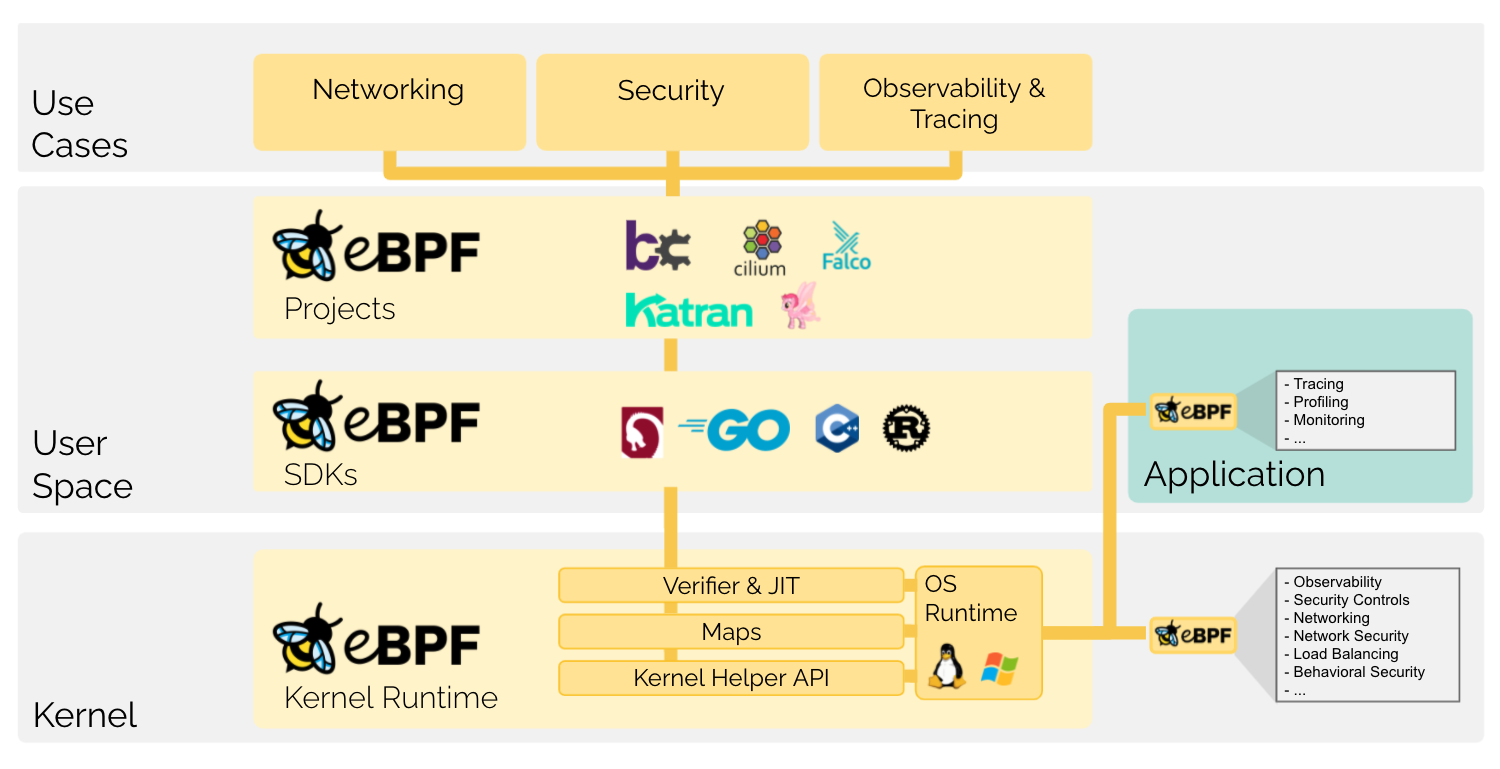
\includegraphics[width=0.8\linewidth]{ebpf-diagram.png}
  \caption{A generic overview of eBPF, from \cite{ebpf}}
  \label{fig:ebpf-generic-overview}
\end{figure}

Some of the most common use cases for eBPF include the implementation of networking, security, and
observability of programs. These are usually implemented in the operating system because of the kernel's
privileges, but the kernel itself is hard to evolve.
On the other hand, application developers can run eBPF programs in order to add additional capabilities at runtime,
and then the operating system guarantees security and efficiency as if natively compiled
by using a Just-In-Time compiler.

These eBPF programs are event-driven and run when a certain hook point is passed. Some
predefined hooks include system calls, network events, and so on. If a hook does not exist,
it is possible to create custom kernel or user probes. An example of how eBPF interacts with the
Linux kernel is visible in Figure \ref{fig:example-ebpf-hooks}.

\begin{figure}[h]
  \centering
  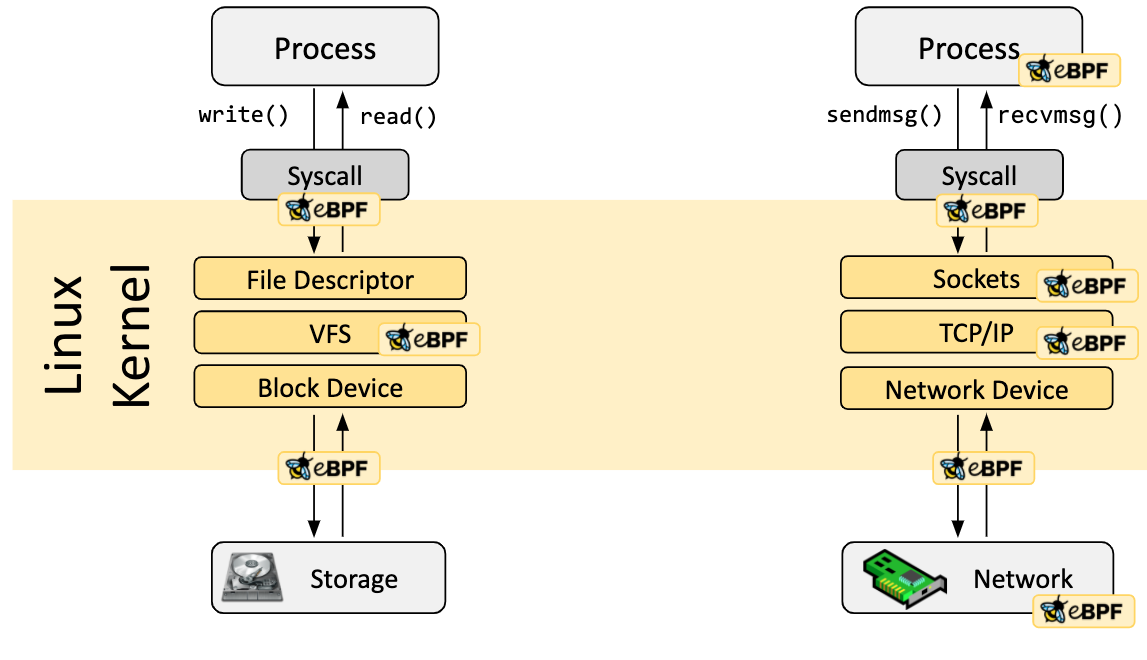
\includegraphics[width=0.8\linewidth]{ebpf-hooks.png}
  \caption{An example of two eBPF hooks, from \cite{ebpf-description}}
  \label{fig:example-ebpf-hooks}
\end{figure}

When running a program with eBPF, there are many steps that are taken:
\begin{enumerate}
  \item first of all, eBPF is usually not used directly but via libraries that provide the ability to specify
        intent-based operations which are then implemented with eBPF; in any case, an eBPF program must be
        compiled into a specific eBPF bytecode;
  \item when a certain \textit{hook} is invoked, this hook has to be identified and then the program can be loaded
        into the kernel with a system call;
  \item a \textit{verification} step ensures that the eBPF program is safe to run by validating a set of conditions
        (e.g., the program has the required capabilities, the program always runs to completion, etc.);
  \item finally, the generic bytecode is then Just-In-Time \textit{compiled} into the machine instructions
        to run the program as efficiently as possible.
\end{enumerate}

Unlike Landlock, eBPF makes it possible to define specific exception, e.g., denying
certain access rights on specific files while allowing them on the containing directory.
It also allows to specify whether a program has access to devices such as \texttt{terminal}
and \texttt{dev}.
Thanks to \texttt{BPFContain} \cite{bpfcontain}
it is also possible to run a container security daemon by leveraging eBPF.  In this case,
specific policies must be written for desired commands.

  \chapter{Enforce the WASI sandbox with LSMs}
  \section{Goals}

The main goal of using \textit{Linux Security Modules} in combination with WebAssembly
is to provide a finer grain customisation when choosing how to limit the permissions given
to the executable. More specifically, the desired features are:
\begin{enumerate}
  \item to give the possibility to differentiate between directories and files when giving permissions;
  \item to clearly separate different capabilities;
  \item to extend the possible set of permissions under the user's control.
\end{enumerate}

Additional desirable features include the possibility to apply exceptions to a certain rule, as well
as limiting the access to other resources in the operating systems, such as network, devices, and
inter-process communications.

Finally, usability is also taken into consideration, especially from the point of view of a user.

Note that the main purpose of these tests is not to replicate all the functionalities given by
the WebAssembly runtimes (\textit{Wasmtime} and \textit{Wasmer}), but to see how their basic features,
especially running a WebAssembly compiled binary through WASI, can be integrated and/or extended with
security tools from the Linux kernel.
This means that, for example, running a single function exported from a WebAssembly module won't be taken
into consideration.

\newpage
\section{Landlock}

For the integration with Landlock, a new project was developed, in order to provide
a custom command line interface that allowed the user to specify with more precision what
the WebAssembly binary is permitted to do on certain folders and files.

The project is open source and the code is available at \url{https://github.com/micheleberetta98/rust-wasm-landlock}.

\subsection{Code architecture and description}\label{sec:landlock-code-architecture}

The code itself is written in \textit{Rust}, and makes use of the
\textit{rust-landlock}\footnote{\url{https://github.com/landlock-lsm/rust-landlock}} crate
to communicate with Landlock and the \textit{wasmtime} and \textit{wasmtime-wasi} official
crates in order to have a runtime environment to execute a WebAssembly binary.

The project is divided into five modules, which are:
\begin{enumerate}
  \item \texttt{args}, used to define and parse the command line arguments that specify the WebAssembly binary,
        the directories to preopen, and the allowed privileges on individual folders and/or files;
  \item \texttt{landlock}, which handles the creation and update of the permissions' ruleset;
  \item \texttt{main}, the module that interfaces with the user;
  \item \texttt{path\_access}, containing a helper structure to track permission for a single path;
  \item and finally \texttt{wasm}, that communicates with the \textit{wasmtime-wasi} and the \textit{wasmtime} crates
        in order to run the provided binaries, as well as preopening directories.
\end{enumerate}

\begin{figure}[ht]
  \centering
  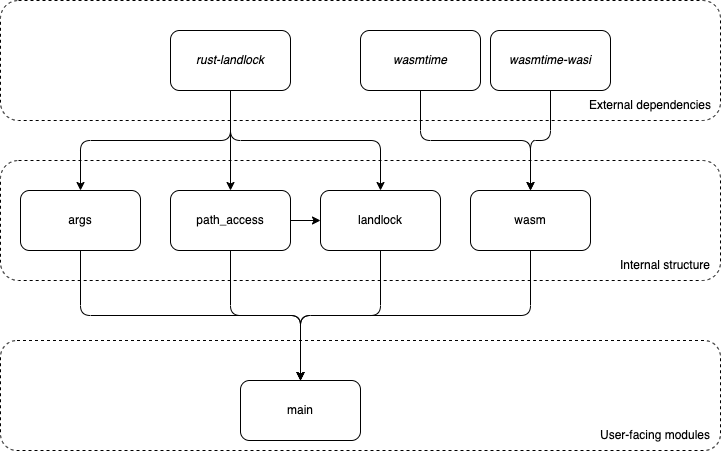
\includegraphics[width=0.9\linewidth]{rust-landlock-code-diagram.png}
  \caption{The code's architecture}
  \label{fig:rust-landlock-code-architecture}
\end{figure}

The architecture diagram is visible in Figure \ref{fig:rust-landlock-code-architecture}, where
are outlined the most important external crates and all dependencies between the modules, represented
by directed arrows.

\subsubsection{The \texttt{args} module}
\label{sec:landlock-args-module}

The main definition of this module is the \texttt{Args} struct, visible in Listing \ref{lst:arg-struct},
used to represent the command line interface that allows to specify which permissions to enable
for one or more specific paths.

\begin{code}[language=rust, caption=The \texttt{Args} struct, label=lst:arg-struct]
  #[derive(Parser, Debug)]
  #[clap(author, version, about, long_about = None)]
  pub struct Args {
    // The module to execute
    pub wasm_module: String,

    // The preopened dir(s) to pass to wasmtime
    pub dirs: Vec<String>,

    // The preopened mapped dir(s) to pass to wasmtime
    pub mapdirs: Vec<(String, String)>,

    // A list of the allowed privileges on a particular folder/file
    pub fs_allows: Vec<(String, BitFlags<AccessFs>)>,

    // Disable landlock (test only)
    pub no_landlock: bool,
  }
\end{code}

Every single field is mapped to one command line argument thanks to the \textit{clap} crates which handles the
creation and parsing of the CLI arguments structure.
Their usage and meaning is described in Table \ref{table:landlock-cli-args}.

Note that here preopening a directories does not mean it and its contents will be accessible by the
provided binary at runtime - they can still be restricted by the landlock policies. Preopening is
necessary though in order to give the possibility to access its contents.

Directories can also be \textit{mapped} - in a way similar to the one provided by the \textit{Wasmtime} command line tool,
it is possible to remap path, so that it's possible to have the binary access any arbitrary path in the system
without manually copying and/or executing it in a specific directory.

\begin{table}
  \centering
  \begin{tabular}{|l|l|l|l|}
    \hline
    \textit{Argument} & \textit{Required} & \textit{Description} \\
    \hline\hline
    \textit{WASM module} & Yes & The path to the WASM binary to run \\ \hline
    \texttt{dir} & No & All the directories to preopen \\ \hline
    \texttt{mapdir} & No & Eventual mappings between the directories \\ \hline
    \texttt{fs-allow} & No & All the permitted actions on a single path \\ \hline
    \texttt{no-landlock} & No & Used to disable the self restriction done by landlock \\
    \hline
  \end{tabular}
  \caption{All the available command line arguments}
  \label{table:landlock-cli-args}
\end{table}

The first argument is positional, and is the path where the WebAssembly module is located.

The arguments \texttt{dir}, \texttt{mapdir} and \texttt{fs-allow} can appear multiple times (or no times at all), and all the values
are then collected into a single \texttt{Vec}. In this way, it is possible to apply different restrictions on different
paths - for example, one could set some files as read-only, while another subset of files in a specific directory
could also be writable.

The \texttt{fs-allow} is made up of two parts, separated by a colon - a path to apply the restrictions to,
and a series of enabled permissions on that specific path, separated by a comma.
Each permission is mapped one-to-one to the flags provided by Landlock in a manner listed in Table \ref{table:landlock-flags}.
Moreover, there are three useful ``shortcuts'' used to represent common situations - \texttt{$\sim$read}, \texttt{$\sim$write} and \texttt{*}.

Lastly, the \texttt{no-landlock} argument is only for testing purposes - it is off by default, so that
landlock is enabled and self restriction is applied if not explicitly disabled.

\subsubsection{The \texttt{wasm} module}

This module manages a single WebAssembly binary module and forms a bridge to the \textit{wasmtime} and the \textit{wasmtime-wasi}
crates. In this project, \textit{Wasmtime} bindings are used instead of the \textit{Wasmer} ones, but both provide the
same level of functionality, albeit with a different interface.

\begin{code}[language=Rust, caption=The outline of the \texttt{wasm} module]
  pub struct WasmModule {
    bytes: Vec<u8>, ctx_builder: WasiCtxBuilder,
  }
  
  impl WasmModule {
    // Reads the WASM module and initialises the WasiCtxBuilder
    pub fn new(path: &str) -> Result<Self> {...}
  
    // Make inherit stdio to the WASM module
    pub fn use_stdio(mut self) -> Self {...}
  
    // Preopen all given directories
    pub fn preopen_all(
      mut self,
      dirs: &Vec<String>) -> Result<Self> {...}
  
    // Preopen and map all given directories
    pub fn preopen_all_map(
      mut self,
      mapdirs: &Vec<(String, String)>) -> Result<Self> {...}
  
    // Preopen (and map) a single directory
    pub fn preopen(
      mut self,
      dir: &str, guest_path: &str) -> Result<Self> {...}
  
    // Run the module
    pub fn run(self) -> Result<()> {...}
  }  
  \end{code}

Here a WASM binary is represented by a vector of bytes, and it is also handled the creation
and construction of a \textit{WASI Context}, a structure defined by the \textit{wasmtime-wasi} crate used to store
all preopened directories, eventual imports and more that will be useful to run the WebAssembly module.

Here are defined various helpers to preopen directories, both unmapped and mapped.
Most importantly, in this module it's defined how to run a WebAssembly binary - it must defined both an \textit{engine} and a \textit{linker},
as well as a \textit{store} which represents the memory of a WebAssembly module described in the previous chapter.

Note that the WebAssembly module has to have a \textit{default exported function} to run - when compiling with a WASI target,
this is usually represented by the \texttt{\_start} function, which corresponds to the \texttt{main} function in languages
such as C and Rust.

\subsubsection{The \texttt{landlock} and \texttt{path\_access} modules}

The \texttt{landlock} module is a thin wrapper around the API made available by the \textit{rust-landlock} crate.
It handles mostly ruleset creation, rule insertion, and enforces the policies before the desired WASM module is run.
The main outline of the code is visible in Listing \ref{lst:rust-landlock}.

\begin{code}[language=Rust, caption=The outline of the \texttt{landlock} module, label=lst:rust-landlock]
  pub struct Landlock {
    ruleset: RulesetCreated,
  }
  
  impl Landlock {
    // Creates a new ruleset with flags from Landlock ABI version 1
    pub fn new() -> Result<Self, RulesetError> {...}
  
    // Add a set of rules to the ruleset
    pub fn add_rules(
      mut self,
      rules: impl Iterator<Item = PathAccess>) -> Result<Self>
    {...}
  
    // Add a single rule to the ruleset
    pub fn add_rule(
      mut self,
      path_access: PathAccess) -> Result<Self>
    {...}
  
    // Self restrict the process and checks whether Landlock
    // is supported or not by the running kernel
    pub fn enforce(self) -> Result<RestrictionStatus> {...}
  }
  \end{code}

It makes use of another thin wrapper, the \texttt{PathAccess} struct defined in the \texttt{path\_access} module.
In this module, the main entity is the \texttt{PathAccess} struct, that tracks which flags as defined in Table \ref{table:landlock-flags}
are applied to a single path. The flags list starts empty, and multiple flags can be added at any times.
Moreover, this module also takes care of conversions between types required by the Landlock ABI in order
to make the code compile.

\subsection{Available permission settings}

The program allows to specify all access right flags from the first version of the Landlock
ABI\footnote{At the moment it is not possible to specify the \texttt{LANDLOCK\_ACCESS\_FS\_REFERER} in order to reparent a file hierarchy.}.

\begin{table}
  \centering
  \begin{tabular}{|l|l|}
    \hline
    \textit{Flag} & \textit{Enabled permission} \\ \hline\hline
    \texttt{X} & Execute a file \\ \hline
    \texttt{W} & Write to a file \\ \hline
    \texttt{R} & Read a file \\ \hline
    \texttt{RDir} & Open a directory or list its content \\ \hline
    \texttt{DDir} & Delete an empty directory or rename one \\ \hline
    \texttt{D} & Unlink or rename a file \\ \hline
    \texttt{MChar} & Create, rename or link a character device \\ \hline
    \texttt{MDir} & Create or rename a directory \\ \hline
    \texttt{MReg} & Create, rename or link a regular file \\ \hline
    \texttt{MSock} & Create, rename or link a socket \\ \hline
    \texttt{MFifo} & Create, rename or link a named pipe \\ \hline
    \texttt{MBlock} & Create, rename or link a block device \\ \hline
    \texttt{MSym} & Create, rename or link a symbolic link \\ \hline
    \texttt{$\sim$read} & Combination of \texttt{X}, \texttt{R} and \texttt{RDir} \\ \hline
    \texttt{$\sim$write} & Combination of all but \texttt{X}, \texttt{R} and \texttt{RDir} \\ \hline
    \texttt{*} & Enable all flags \\ \hline
  \end{tabular}
  \caption{Provided flags and corresponding Landlock permissions}
  \label{table:landlock-flags}
\end{table}

All flags are listed in Table \ref{table:landlock-flags}, and some the following examples illustrate how to combine them:
\begin{itemize}
  \item \texttt{file:R} allows only to read from \textit{file};
  \item \texttt{file:X} the combination of \texttt{.:RDir} allows the execution of \textit{file} and the listing of the current directory;
  \item \texttt{.:MReg} only allows the creation, rename or linking of regular files in the current directory;
  \item \texttt{.:R,W} and \texttt{./subdir:*} allows only reads and writes on files in the current directory, while no restrictions are
        made for \textit{subdir}.
\end{itemize}

Note that, as highlighted in Section \ref{sec:landlock-args-module}, the directories containing the files of interest
must always be preopened, even if their content is then restricted by landlock.

The Landlock self-restriction is applied after the necessary preopening of the directories,
otherwise the running process would have to always have the permissions for listing directories even if
not needed by the WASM binary.

\subsection{Advantages and disadvantages}

The main advantage that Landlock brings is simplicity. For the developer, the API is simple enough to use
to use, and it can be used in a variety of languages - the main two languages are C (used directly with the kernel libraries),
Rust as in this project, and Go\footnote{\url{https://github.com/landlock-lsm/go-landlock}}.
From the user's point of view, the provided permission flags are clear enough that it is not required to have
anything beside a basic understanding of Linux's file system permissions.
Hence, it can be used to provide a clear interface that is not so different from the one already given by
the existing runtimes.
Moreover, Landlock allows \textit{unprivileged} access control - it is not necessary to gain particular privileges
when running a binary, so the user can run a WebAssembly module in a protected environment even if they are not
in the \textit{sudoers} group.

The biggest drawback with this approach is simplicity itself. As highlighted in Section \ref{sec:intro-lsm-landlock},
there is no way to define exception - this restricts the possibilities given to the user, and makes some situations
impossible to specify. For example, if a \texttt{LANDLOCK\_ACCESS\_FS\_REMOVE\_FILE} right is given to a directory,
all files in that directory can be renamed and there is no way to prevent renaming for a specific file.
Or similarly, if a \texttt{LANDLOCK\_ACCESS\_FS\_READ\_DIR} right is given to a directory, all subdirectories
will be subjected to the same access right, so it is not possible to discriminate between subdirectories.
In addition to this, the set of capabilities is somewat limited, and mostly related to the file system.

\section{eBPF with \textit{bpfcontain}}

\subsection{Architecture}

\subsection{Available permission settings}

\subsection{Advantages and disadvantages}

  \chapter{Performance}
  \section{Testing plan}

The main goals of this performance testing plan are:
\begin{itemize}
  \item to find out whether the usage of LSM implies some sort of performance penalty;
  \item to identify possible improvements when embedding WebAssembly in another language.
\end{itemize}

\noindent
For a given program written in Rust, the following configurations are tested:
\begin{itemize}
  \item a native binary, compiled by \texttt{rustc} and run as an executable under the following conditions:
        \begin{itemize}
          \item without a sandbox;
          \item sandboxed with Landlock (in this case, the program has to be modified - an example is visible in Listing \ref{lst:test-program-landlock-example});
          \item sandboxed with eBPF.
        \end{itemize}
  \item a WebAssembly binary obtained by the same Rust program and run:
        \begin{itemize}
          \item directly by the \textit{Wasmtime} command line tool;
          \item by the WASM runtime developed in Section \ref{sec:restricting-wasi-landlock} and restricted with Landlock;
          \item by the WASM runtime developed in Section \ref{sec:restricting-wasi-landlock} and restricted with
                eBPF\footnote{In this case, Landlock is disabled.}.
        \end{itemize}
\end{itemize}

\vspace*{0.5cm}
\begin{code}[language=Rust, caption=An example of a program restricted with Landlock., label=lst:test-program-landlock-example]
use anyhow::Result;
use landlock::*;

const ACCESS: BitFlags<AccessFs> =
  make_bitflags!(AccessFs::{ ReadFile });

fn main() -> Result<()> {
    let path_fd = PathFd::new("input-file.txt")?;
    
    let path_beneath = PathBeneath::new(path_fd)
      .allow_access(ACCESS);
    let _ = Ruleset::new()
        .handle_access(AccessFs::from_all(ABI::V1))?
        .create()?
        .add_rule(path_beneath)?
        .restrict_self()?;

    // Here goes the main code
    // ...

    Ok(())
}
\end{code}

\clearpage
\subsection{System and hardware}

The system and hardware used for both the development of the project described in Section \ref{sec:restricting-wasi-landlock}
and the performed test is as follows:
\begin{itemize}
  \item Arch Linux \cite{arch-linux} as the operating system, more specifically the 2022.05.01 version;
  \item an Intel Core i5-7200U quad-core with a clock rate of 2.5 GHz;
  \item 8 GB of RAM;
  \item a 120 GB solid state disk.
\end{itemize}

The choice of the operating system is mainly dictated by the fact that Arch Linux has both Landlock and eBPF active
out of the box, removing the need to compile the Linux kernel with the necessary flags to enable these
functionalities.

\subsection{Tests' description}
\label{sec:performance-test-description}

The performed tests are:
\begin{itemize}
  \item a purely computational program, given by the sorting of 10000 random numbers as in Listing \ref{lst:sorting-test-rust},
        in order to measure only the computational impact of the various methods;
  \item a simple reading of files of various sizes as in Listing \ref{lst:reading-test-rust}, with only the necessary permissions enabled on
        a case-by-case bases, in order to test the sandbox provided and how they fare against native binaries.
\end{itemize}

The reading file test is repeated with different file sizes\footnote{Randomly generated by using \texttt{/dev/urandom}.},
which are $100$ KB, $1$ MB, $10$ MB and $100$ MB. By doing this, it is possible to see how performance
varies when dealing with progressively large files. Moreover, an additional empty file is used to
test the overhead on the pure opening of a file.

\vspace*{0.5cm}
\begin{code}[language=Rust, caption=The tested ``sorting program''., label=lst:sorting-test-rust]
use rand::Rng;

fn main() {
  let mut rng = rand::thread_rng();
  let mut vec: Vec<i32> = Vec::new();

  for _ in 0..10000 {
    vec.push(rng.get::<i32>());
  }

  vec.sort();
}
\end{code}

\begin{code}[language=Rust, caption=The tested ``reading program''., label=lst:reading-test-rust]
fn main() {
  let content = std::fs::read("input-file.txt");
  match content {
      Ok(c) => println!("{}", c.len()),
      Err(_e) => std::process::exit(1),
  }
}
\end{code}

\subsection{Performance indicators}

The main performance indicators will be the mean execution time, measured in milliseconds, together with its
standard deviation in order to compensate for variability.
These measures are always obtained from a sample of 100 runs, executed and measured by \texttt{hyperfine},
a command-line benchmarking tools \cite{hyperfine}, and finally saved to a
JSON file.

In this chapter, we define for brevity $\mu_x$ to be the mean of the method $x$ and $\sigma_x$ to be
the standard deviation of the method $x$.

\section{Comparison between different sandboxes}

In this section we will look at what impact different LSMs bring on a program,
be it a native binary or a WebAssembly binary run through some kind of runtime.

In Table \ref{table:lsm-impact-native} are present all execution times for a native binary,
compiled directly with \texttt{rustc} and run both unrestricted (\textit{Native}) and restricted
with different LSMs (\textit{Landlock} and \textit{eBPF}).

On the other hand, Table \ref{table:lsm-impact-wasm} is about running a WebAssembly binary through
\textit{Wasmtime} without any restriction, or through the WASM runtime developed in Section \ref{sec:restricting-wasi-landlock}
and restricted with Landlock (\textit{WL}) or eBPF (\textit{WeBPF}).

\begin{table}
  \centering
  \csvreader[
    tabular={|l|r|r|r|r|r|r|},
    table head = \hline
      \textit{Test type}
      & $\mu_\mathrm{Native}$   & $\sigma_\mathrm{Native}$
      & $\mu_\mathrm{Landlock}$ & $\sigma_\mathrm{Landlock}$
      & $\mu_\mathrm{eBPF}$     & $\sigma_\mathrm{eBPF}$ \\ \hline\hline,
    late after line = \\ \hline,
    head to column names,
  ]{test-data/native-landlock-ebpf.csv}{}
  {\type & \mnative & \snative & \mlandlock & \slandlock & \mebpf & \sebpf}
  \caption{Execution times of a native binary under different restrictions (in ms).}
  \label{table:lsm-impact-native}
\end{table}

\begin{table}
  \centering
  \csvreader[
    tabular={|l|r|r|r|r|r|r|},
    table head = \hline
      \textit{Test type}
      & $\mu_\mathrm{Wasmtime}$   & $\sigma_\mathrm{Wasmtime}$
      & $\mu_\mathrm{WL}$ & $\sigma_\mathrm{WL}$
      & $\mu_\mathrm{WeBPF}$     & $\sigma_\mathrm{WeBPF}$ \\ \hline\hline,
    late after line = \\ \hline,
    head to column names,
  ]{test-data/wasm-landlock-ebpf.csv}{}
  {\type & \mnative & \snative & \mlandlock & \slandlock & \mebpf & \sebpf}
  \caption{Execution times of a WASM binary under different restrictions (in ms).}
  \label{table:lsm-impact-wasm}
\end{table}

\subsection{A computational-heavy program}

Let's take a look at how restricting a purely computational-heavy program, namely the sorting of 
10000 random numbers showin in Listing \ref{lst:sorting-test-rust}, affects its performance.
In order to test the eBPF sandbox, Listing \ref{lst:outline-policy-sorting-test} shows the outline for the used policy.

Comparing the first lines of Table \ref{table:lsm-impact-native} and Table \ref{table:lsm-impact-wasm},
it is immediately apparent that using a LSM to restrict a binary, be it native or WebAssembly, worsen performance.

When dealing with a native binary, \textit{Landlock} has a lower overhead than \textit{eBPF} (an average
of $1.03$ ms for Landlock against an average of $2.30$ for eBPF), as is visible in Figure \ref{fig:distribution-sorting-native}.
This could be due to how the two sandoxes are enforced:
\begin{itemize}
  \item Landlock is directly available as a C library in the Linux kernel, so the communication between
        the program and the relative LSM can be as simple as multiple function calls;
  \item on the other hand, eBPF needs to have an active server\footnote{As highlighted in Section \ref{sec:restricting-wasi-ebpf}.},
        so the communication has to undergo a message exchange between processes.
\end{itemize}
By following this line of reasoning, it is expected that Landlock should be a little faster than eBPF.
Moreover, eBPF is more complex than Landlock since it allows more control on what
can and cannot be done by a running program, hence it has to deal with a higher complexity.
The overhead of eBPF, however, becomes smaller and smaller when measured in percentage as the execution times get higher.
This means that for small and fast programs the slow-down could become apparent if they get called many times
in a short period of time, while for slower program called with less frequency this should be negligible.

\vspace*{0.5cm}
\begin{code}[language=yaml, caption=The outline of the policy used for testing the sorting program., label=lst:outline-policy-sorting-test]
name: test-sorting
cmd: # The command to be executed
allow:
- fs: {pathname: ., access: rxm}
\end{code}

When dealing with a WebAssembly binary, the computational-heavy program is noticeably slower
compared to the native binary execution times, either unrestricted or restricted, as shown in Figure
\ref{fig:distribution-sorting-wasm}\footnote{Note that Figures \ref{fig:distribution-sorting-wasm} and \ref{fig:distribution-sorting-native}
have different scales.}.
The same reasoning applied before is valid here too - eBPF is a little slower than Landlock, with a overhead
of about $1$ ms.
However, restricting a WASM binary with the runtime developed in Section \ref{sec:restricting-wasi-landlock}
introduces a constant overhead of around $30$ ms with respect to \textit{Wasmtime}.
Since it is visible in Table \ref{table:lsm-impact-native} that Landlock is quite close to
unrestricted performance on average, and because Landlock was disabled when running
the tests combining WASM and eBPF, this extra time could be due to how the WASM module gets
interpreted by the library provided by \textit{Wasmtime}\footnote{This will be analysed more
accurately in Section \ref{sec:performance-internal-analysis}.}.

\begin{figure}[ht]
  \centering
  \begin{subfigure}[b]{0.32\textwidth}
    \centering
    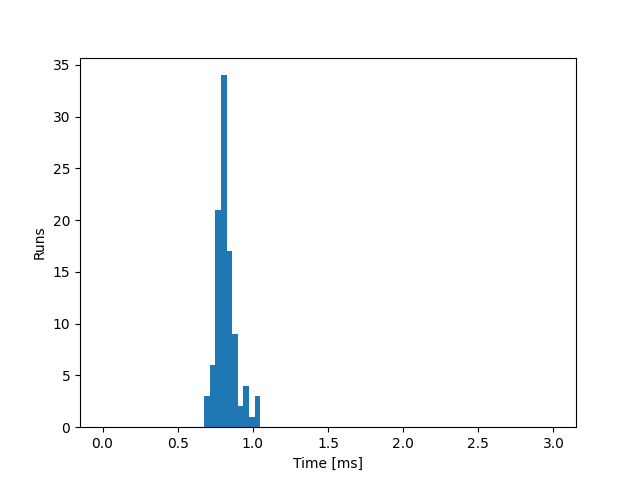
\includegraphics[width=\textwidth]{tests/sorting.native.png}
    \caption{Native}
  \end{subfigure}
  \begin{subfigure}[b]{0.32\textwidth}
    \centering
    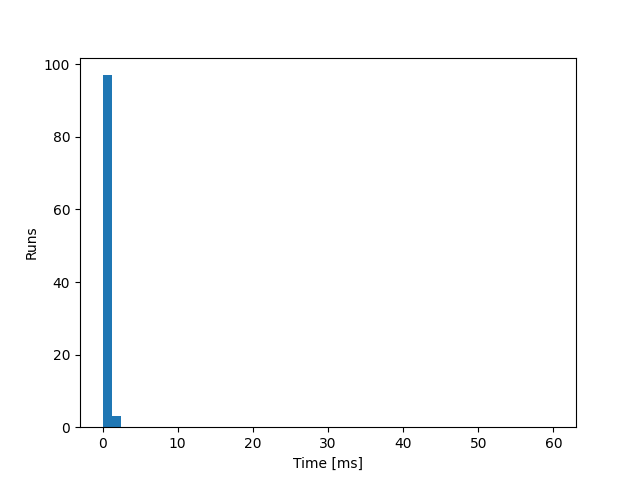
\includegraphics[width=\textwidth]{tests/sorting.native-landlock.png}
    \caption{Landlock}
  \end{subfigure}
  \begin{subfigure}[b]{0.32\textwidth}
    \centering
    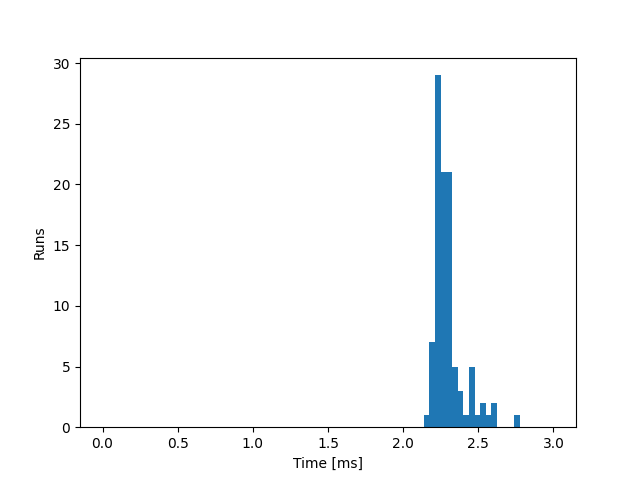
\includegraphics[width=\textwidth]{tests/sorting.native-bpf.png}
    \caption{eBPF}
  \end{subfigure}
  \caption{Distribution of execution times when sorting 10000 numbers (native).}
  \label{fig:distribution-sorting-native}
\end{figure}

\begin{figure}[ht!]
  \centering
  \begin{subfigure}[b]{0.32\textwidth}
    \centering
    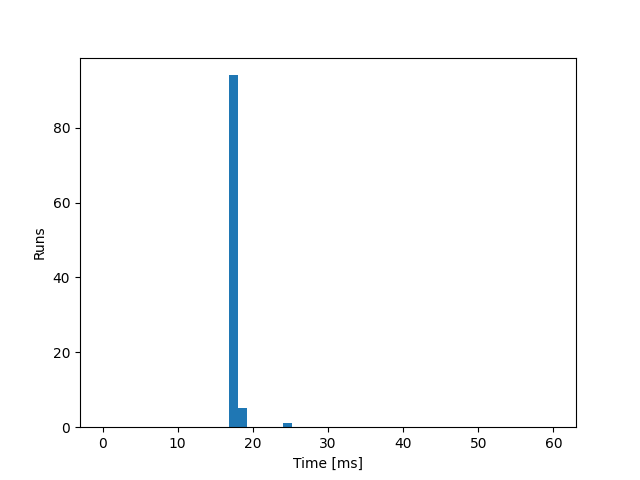
\includegraphics[width=\textwidth]{tests/sorting.wasmtime.png}
    \caption{Wasmtime}
  \end{subfigure}
  \begin{subfigure}[b]{0.32\textwidth}
    \centering
    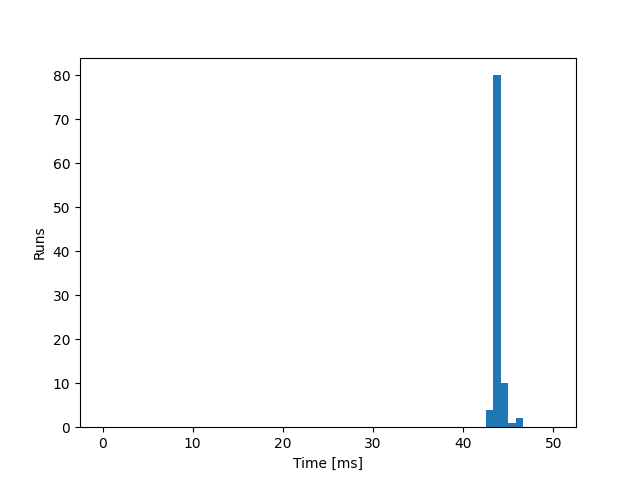
\includegraphics[width=\textwidth]{tests/sorting.wasm-landlock.png}
    \caption{WASM + Landlock}
  \end{subfigure}
  \begin{subfigure}[b]{0.32\textwidth}
    \centering
    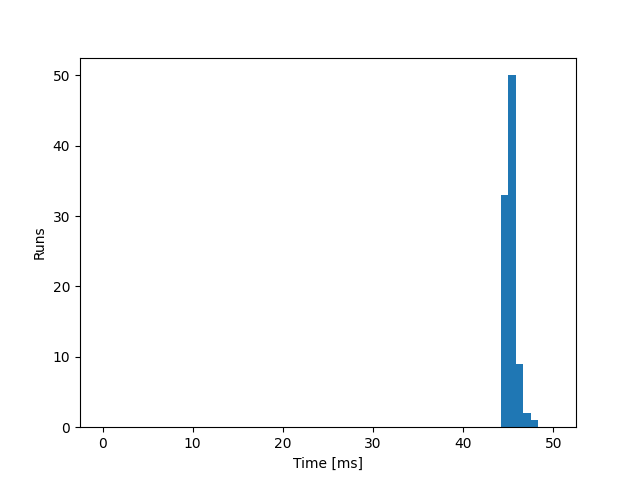
\includegraphics[width=\textwidth]{tests/sorting.wasm-bpf.png}
    \caption{WASM + eBPF}
  \end{subfigure}
  \caption{Distribution of execution times when sorting 10000 numbers (WASM).}
  \label{fig:distribution-sorting-wasm}
\end{figure}

\subsection{File system access}

\begin{figure}[h]
  \centering
  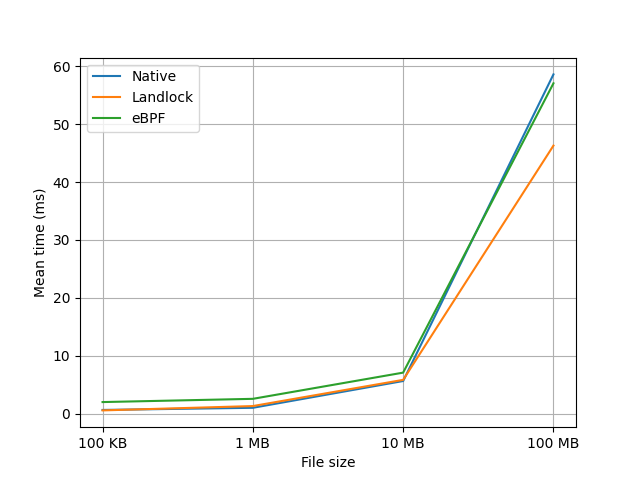
\includegraphics[width=0.8\linewidth]{tests/reading-file-native-graph.png}
  \caption{A comparison of native average speeds when reading a file.}
  \label{fig:avg-comparison-native-speed}
\end{figure}

\begin{figure}[ht!]
  \centering
  \begin{subfigure}[b]{0.32\textwidth}
    \centering
    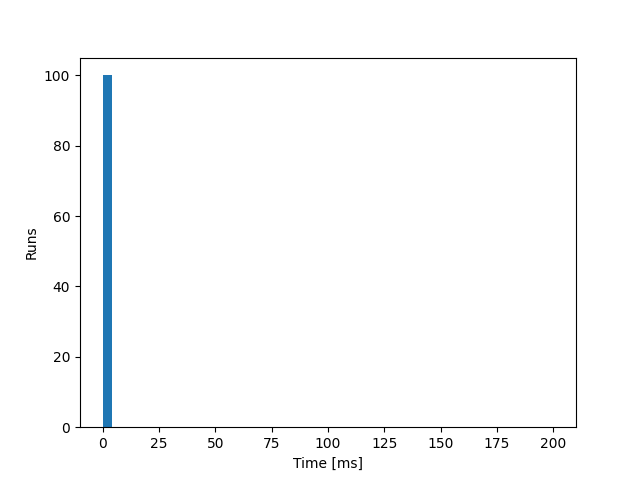
\includegraphics[width=\textwidth]{tests/reading-file-100k.native.png}
    \caption{Native (100 KB)}
  \end{subfigure}
  \begin{subfigure}[b]{0.32\textwidth}
    \centering
    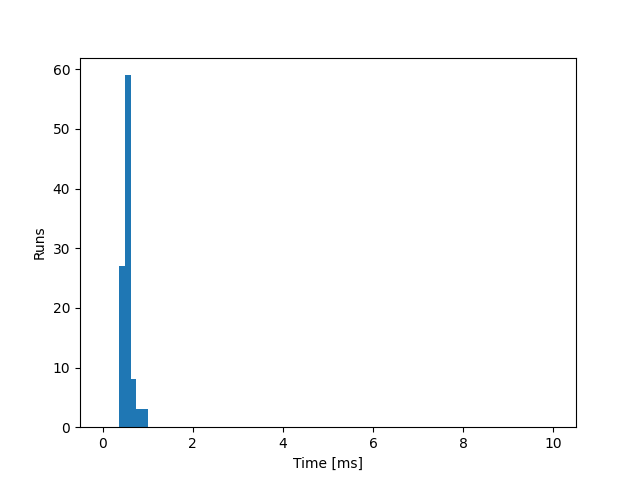
\includegraphics[width=\textwidth]{tests/reading-file-100k.native-landlock.png}
    \caption{Landlock (100 KB)}
  \end{subfigure}
  \begin{subfigure}[b]{0.32\textwidth}
    \centering
    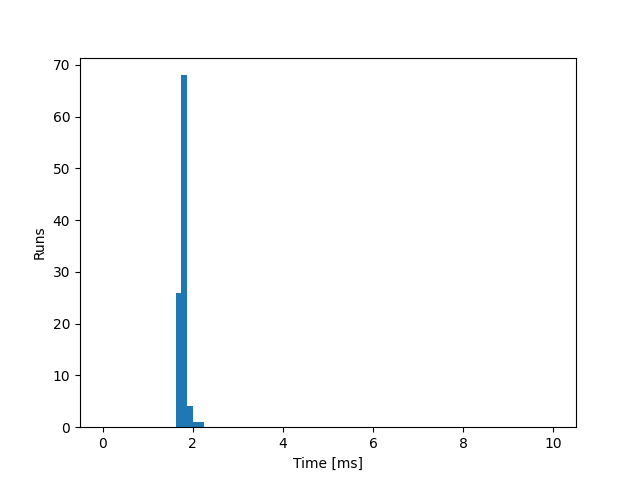
\includegraphics[width=\textwidth]{tests/reading-file-100k.native-bpf.png}
    \caption{eBPF (100 KB)}
  \end{subfigure}

  \begin{subfigure}[b]{0.32\textwidth}
    \centering
    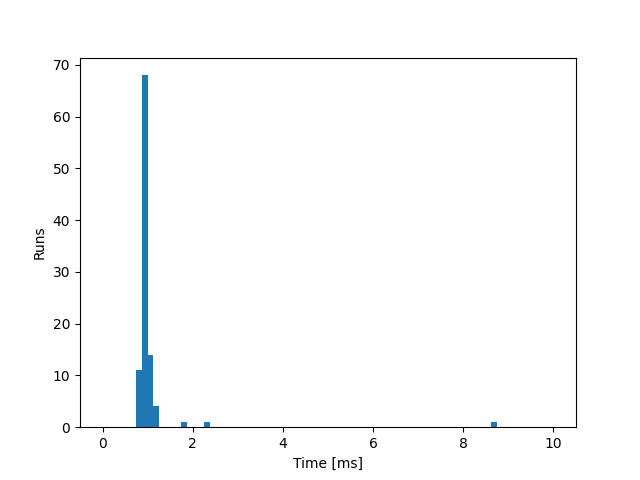
\includegraphics[width=\textwidth]{tests/reading-file-1M.native.png}
    \caption{Native (1 MB)}
  \end{subfigure}
  \begin{subfigure}[b]{0.32\textwidth}
    \centering
    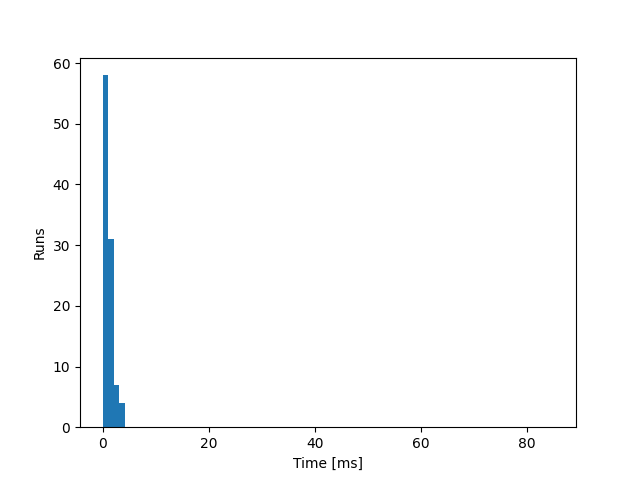
\includegraphics[width=\textwidth]{tests/reading-file-1M.native-landlock.png}
    \caption{Landlock (1 MB)}
  \end{subfigure}
  \begin{subfigure}[b]{0.32\textwidth}
    \centering
    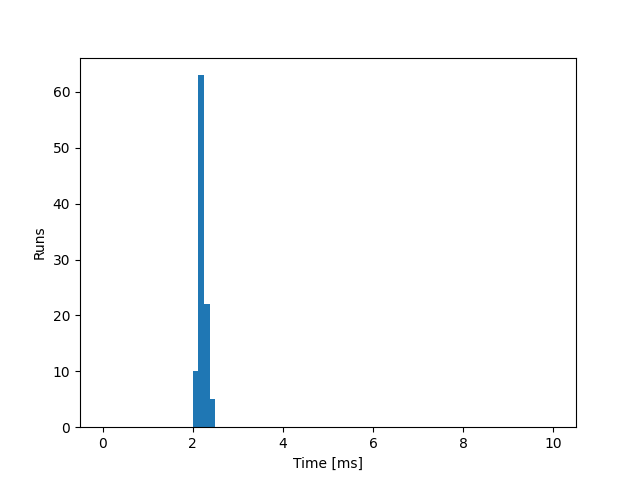
\includegraphics[width=\textwidth]{tests/reading-file-1M.native-bpf.png}
    \caption{eBPF (1 MB)}
  \end{subfigure}

  \begin{subfigure}[b]{0.32\textwidth}
    \centering
    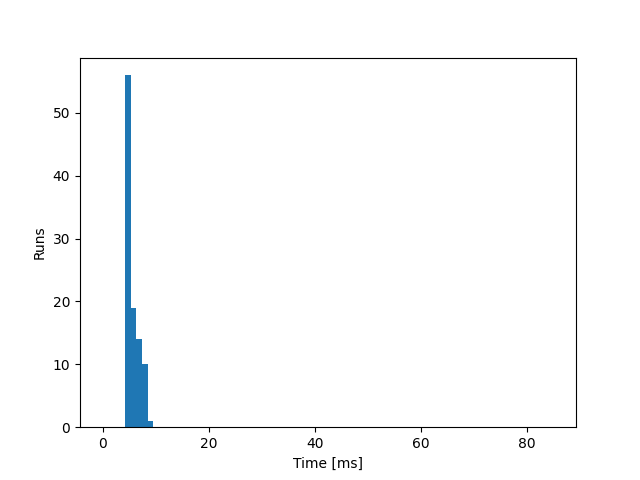
\includegraphics[width=\textwidth]{tests/reading-file-10M.native.png}
    \caption{Native (10 MB)}
  \end{subfigure}
  \begin{subfigure}[b]{0.32\textwidth}
    \centering
    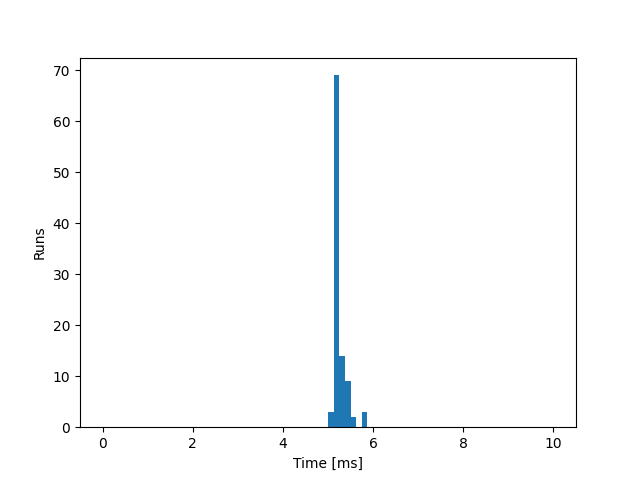
\includegraphics[width=\textwidth]{tests/reading-file-10M.native-landlock.png}
    \caption{Landlock (10 MB)}
  \end{subfigure}
  \begin{subfigure}[b]{0.32\textwidth}
    \centering
    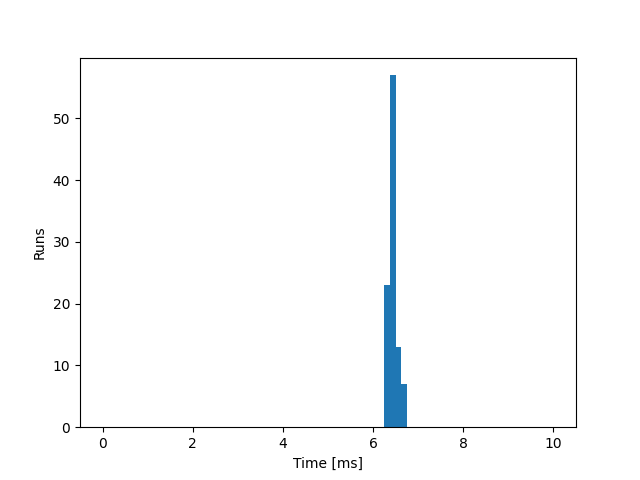
\includegraphics[width=\textwidth]{tests/reading-file-10M.native-bpf.png}
    \caption{eBPF (10 MB)}
  \end{subfigure}

  \begin{subfigure}[b]{0.32\textwidth}
    \centering
    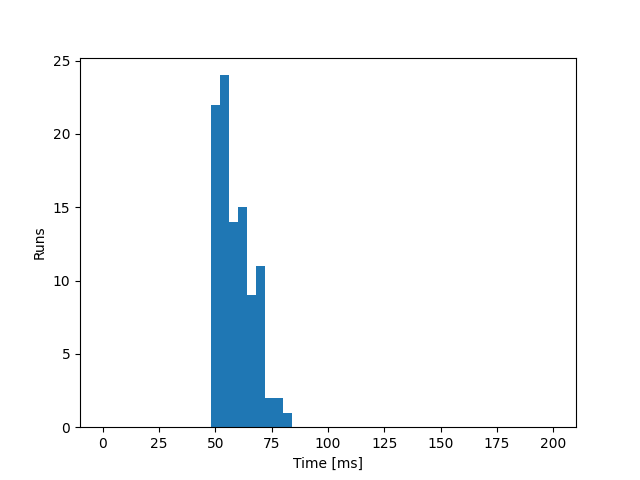
\includegraphics[width=\textwidth]{tests/reading-file-100M.native.png}
    \caption{Native (100 MB)}
  \end{subfigure}
  \begin{subfigure}[b]{0.32\textwidth}
    \centering
    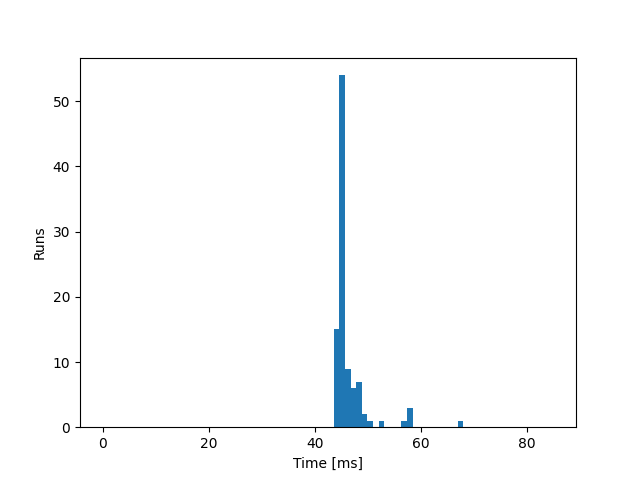
\includegraphics[width=\textwidth]{tests/reading-file-100M.native-landlock.png}
    \caption{Landlock (100 MB)}
  \end{subfigure}
  \begin{subfigure}[b]{0.32\textwidth}
    \centering
    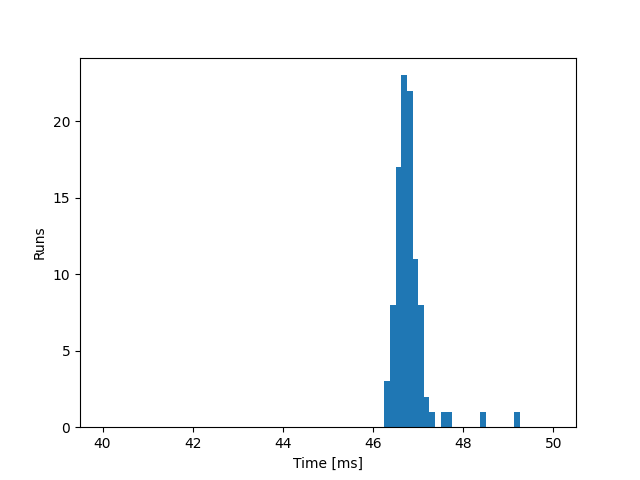
\includegraphics[width=\textwidth]{tests/reading-file-100M.native-bpf.png}
    \caption{eBPF (100 MB)}
  \end{subfigure}

  \caption{Distribution of a native binary execution times when reading a file.}
  \label{fig:distribution-reading-native}
\end{figure}


% The first thing of note, immediately shown by the data in Table \ref{table:lsm-impact-wasm},
% is that on average every single execution of a WASM binary, either restricted or not,
% is slower than running directly a native binary. This is also shown in the three distribution
% graphs visible in Figure \ref{fig:distribution-sorting-wasm}, especially when compared with
% the ones in Figure \ref{fig:distribution-sorting-native}.

% Hence, a WASM binary performance is reasonably comparable to a native binary,
% although there is a constant overhead of at least 20 ms in all the test runs.

% There is another interesting result that presents itself when analysing the integration of Landlock
% and the embedding of WebAssembly modules in Rust (through \textit{Wasmtime}) -
% a constant overhead with respect to using \textit{Wasmtime} directly or through eBPF.
% This can be seen in Table \ref{table:lsm-impact-wasm}, but is more visible in Figure \ref{fig:avg-comparison-wasm-speed},
% showing how the average execution time varies with respect to read file size -
% the \textit{Landlock} curve has roughly the same shape as the other two, but appears translated
% of a constant factor of around 30 ms.

% Since in Section \ref{sec:landlock-vs-ebpf-native} it was shown that no restriction method had a considerable overhead
% against a native binary, and because in this case the WASM module is interpreted by a native binary
% restricted with Landlock, it stands to reason that this overhead should be due to the usage
% of the library provided by \textit{Wasmtime} for integrating WASM in Rust.

% In all cases, however, execution times are not higher than 200 ms - although being a noticeable
% delay, this is small enough to not be of any discomfort to a human user.

\begin{figure}[ht!]
  \centering
  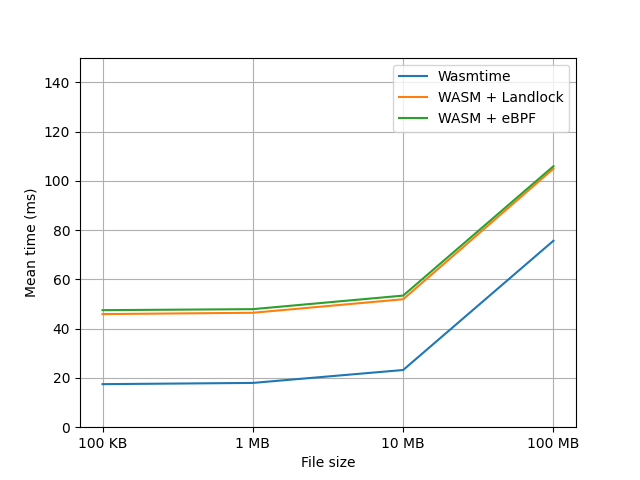
\includegraphics[width=0.8\linewidth]{tests/reading-file-wasm-graph.png}
  \caption{A comparison of WASM average speeds when reading a file.}
  \label{fig:avg-comparison-wasm-speed}
\end{figure}

\begin{figure}[ht!]
  \centering
  \begin{subfigure}[b]{0.32\textwidth}
    \centering
    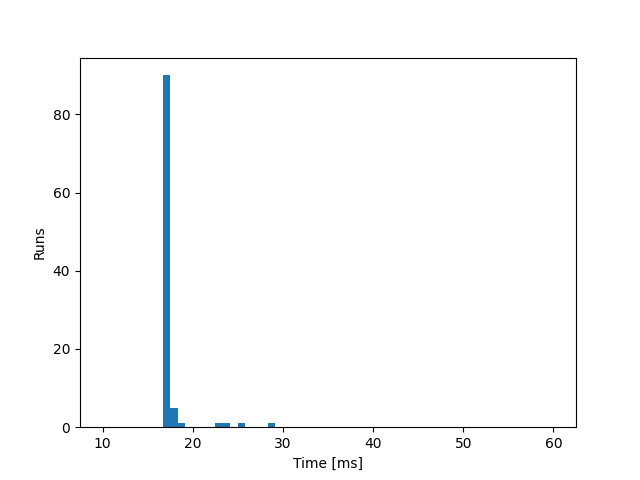
\includegraphics[width=\textwidth]{tests/reading-file-100k.wasmtime.png}
    \caption{Wasmtime (100 KB)}
  \end{subfigure}
  \begin{subfigure}[b]{0.32\textwidth}
    \centering
    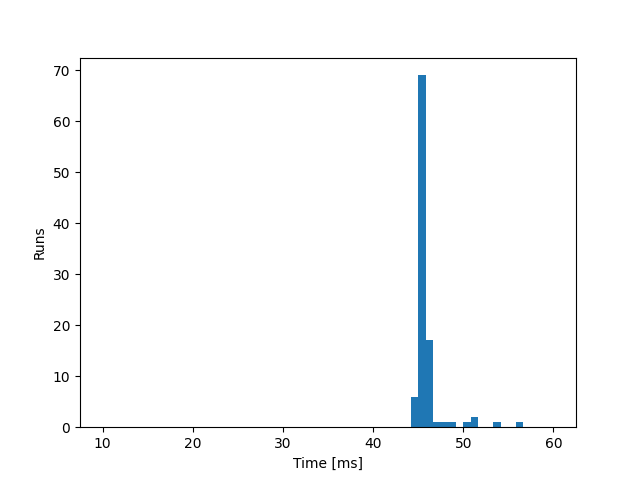
\includegraphics[width=\textwidth]{tests/reading-file-100k.wasm-landlock.png}
    \caption{Landlock (100 KB)}
  \end{subfigure}
  \begin{subfigure}[b]{0.32\textwidth}
    \centering
    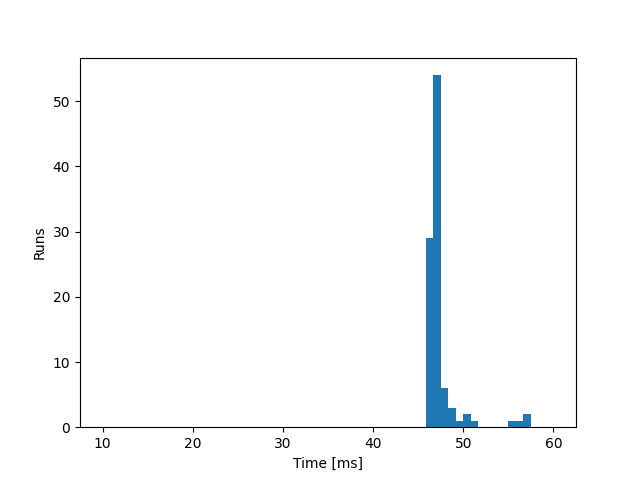
\includegraphics[width=\textwidth]{tests/reading-file-100k.wasm-bpf.png}
    \caption{eBPF (100 KB)}
  \end{subfigure}

  \begin{subfigure}[b]{0.32\textwidth}
    \centering
    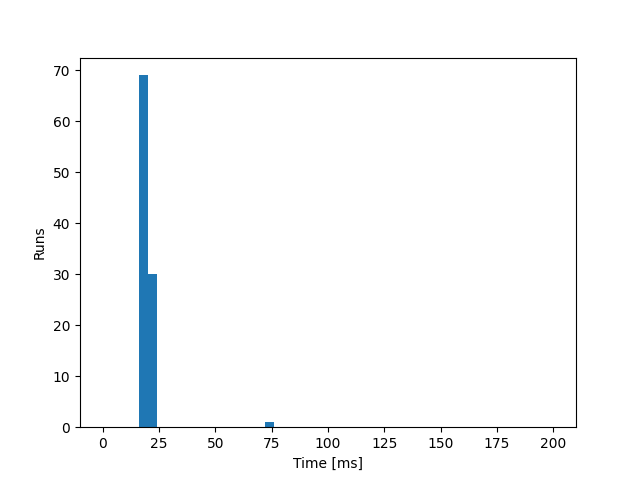
\includegraphics[width=\textwidth]{tests/reading-file-1M.wasmtime.png}
    \caption{Wasmtime (1 MB)}
  \end{subfigure}
  \begin{subfigure}[b]{0.32\textwidth}
    \centering
    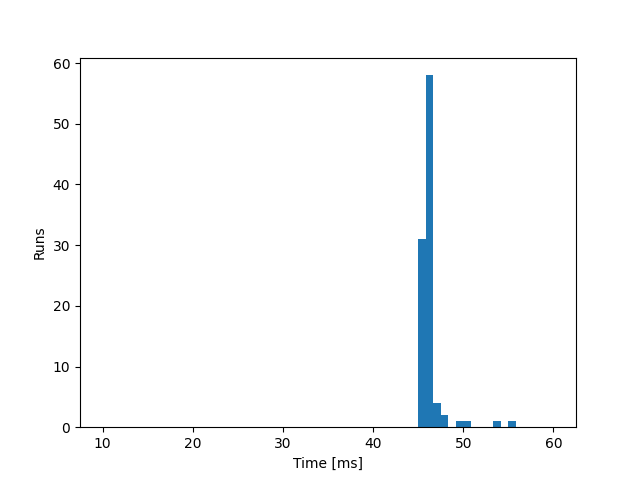
\includegraphics[width=\textwidth]{tests/reading-file-1M.wasm-landlock.png}
    \caption{Landlock (1 MB)}
  \end{subfigure}
  \begin{subfigure}[b]{0.32\textwidth}
    \centering
    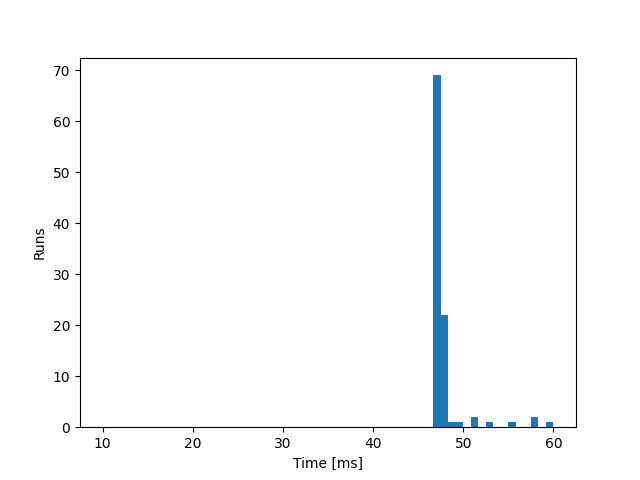
\includegraphics[width=\textwidth]{tests/reading-file-1M.wasm-bpf.png}
    \caption{eBPF (1 MB)}
  \end{subfigure}

  \begin{subfigure}[b]{0.32\textwidth}
    \centering
    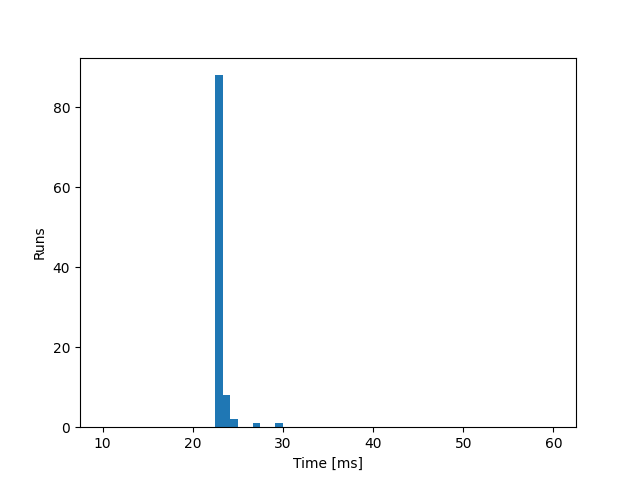
\includegraphics[width=\textwidth]{tests/reading-file-10M.wasmtime.png}
    \caption{Wasmtime (10 MB)}
  \end{subfigure}
  \begin{subfigure}[b]{0.32\textwidth}
    \centering
    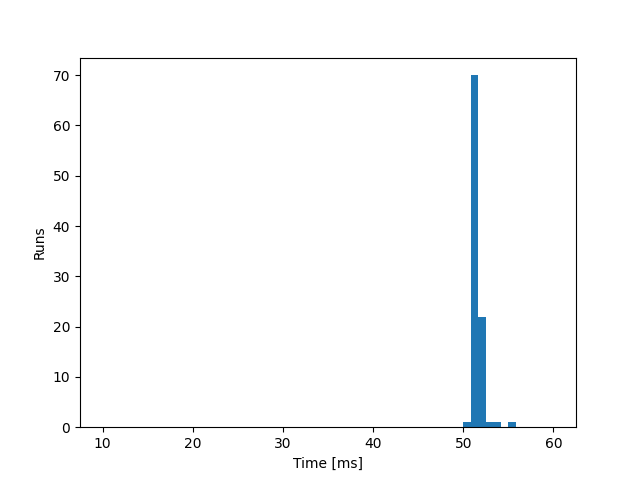
\includegraphics[width=\textwidth]{tests/reading-file-10M.wasm-landlock.png}
    \caption{Landlock (10 MB)}
  \end{subfigure}
  \begin{subfigure}[b]{0.32\textwidth}
    \centering
    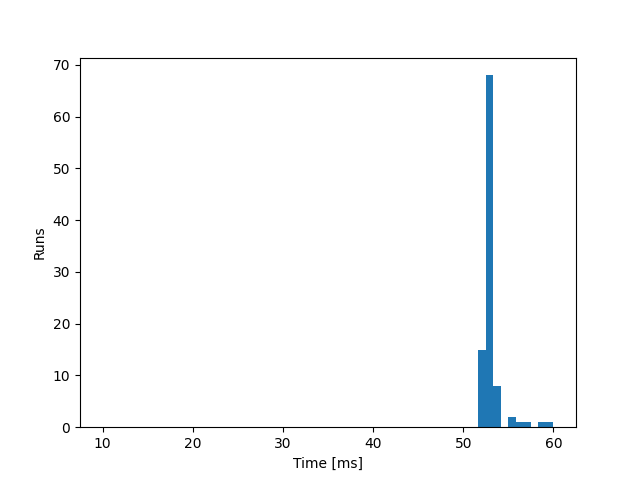
\includegraphics[width=\textwidth]{tests/reading-file-10M.wasm-bpf.png}
    \caption{eBPF (10 MB)}
  \end{subfigure}

  \begin{subfigure}[b]{0.32\textwidth}
    \centering
    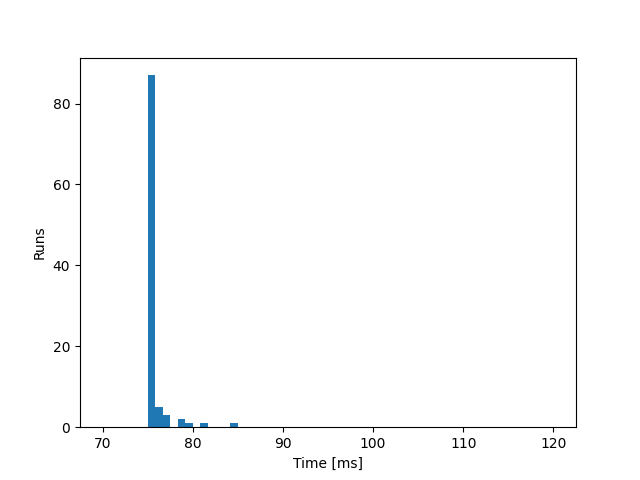
\includegraphics[width=\textwidth]{tests/reading-file-100M.wasmtime.png}
    \caption{Wasmtime (100 MB)}
  \end{subfigure}
  \begin{subfigure}[b]{0.32\textwidth}
    \centering
    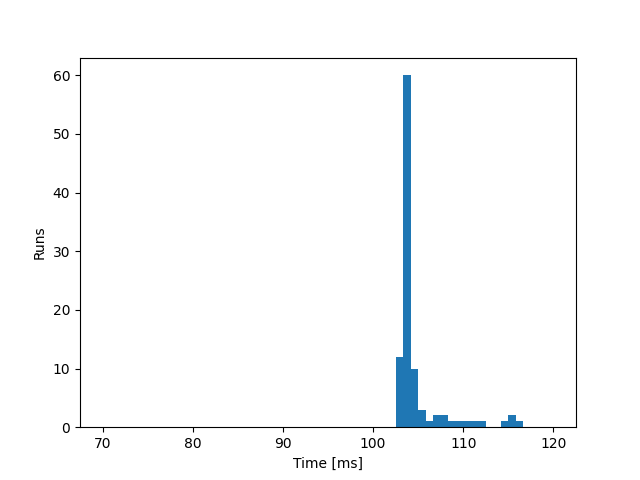
\includegraphics[width=\textwidth]{tests/reading-file-100M.wasm-landlock.png}
    \caption{Landlock (100 MB)}
  \end{subfigure}
  \begin{subfigure}[b]{0.32\textwidth}
    \centering
    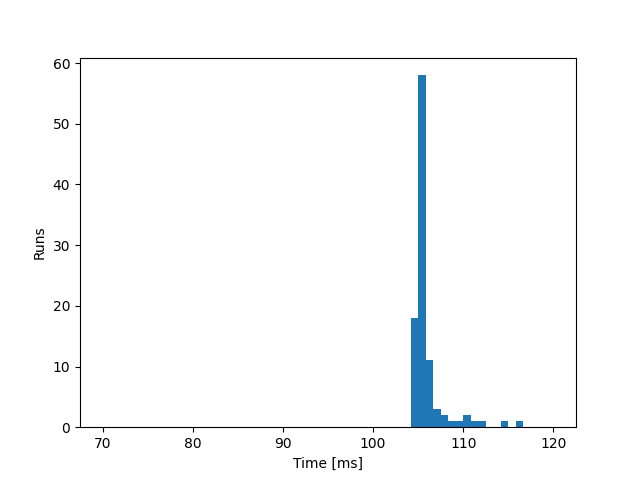
\includegraphics[width=\textwidth]{tests/reading-file-100M.wasm-bpf.png}
    \caption{eBPF (100 MB)}
  \end{subfigure}

  \caption{Distribution of a WASM binary execution times when reading a file.}
  \label{fig:distribution-reading-wasm}
\end{figure}

\section{Internal analysis of the developed project}
\label{sec:performance-internal-analysis}

In order to test the performance of the integration between Landlock and WebAssembly,
embedded in Rust through WebAssembly, through the use of the standard library \texttt{std::time::Instant}
various timestamps were taken and then combined in order to measure the execution time of various program parts.
A total of 100 runs were used in order to measure the average execution times.

Two different WebAssembly programs were tested - a trivial one
(Listing \ref{lst:project-perf-program-simple}) and a more complex one, with
file system access and specific restrictions enabled (Listing \ref{lst:project-perf-program-complex}).
Both these programs were compiled with \texttt{rustc} with a \texttt{wasm32-wasi} target and full
optimisations enabled.

\vspace*{0.5cm}

\begin{code}[language=Rust, caption=The tested trivial program, label=lst:project-perf-program-simple]
  fn main() {
    println!("Hello World");
  }
\end{code}

\clearpage
\begin{code}[language=Rust, caption=The more complex tested program, label=lst:project-perf-program-complex]
use std::fs::{read_to_string, write};

fn main() {
  read_to_string("file1.txt")
    .expect("Could not read file1");
  write("file1.txt", "New content 1")
    .expect("Could not write file1");
  read_to_string("subdir/file2.txt")
    .expect("Could not read file2");
  write("subdir/file2.txt", "New content 2")
    .expect("Could not write file2");
}  
\end{code}

\subsection{Execution times}

The different program parts considered in these measures are the following:
\begin{itemize}
  \item argument parsing;
  \item WASM module instantiation;
  \item the preopening of all directories by Wasmtime;
  \item applying all the Landlock rules;
  \item and finally, compiling and running the WASM module.
\end{itemize}

\begin{table}
  \centering
  \csvreader[
    tabular={|l|r|r|r|r|},
    table head = \hline
      \textit{Program part} & $\mu_\mathrm{Instant}$ & $\sigma_\mathrm{Instant}$ & $\mu_\mathrm{Cumulative}$ & $\sigma_\mathrm{Cumulative}$   \\ \hline\hline,
    late after line = \\ \hline,
    head to column names,
  ]{test-data/project-stats-simple.csv}{}
  {\type & \mean & \stddev & \meanc & \stddevc}
  \caption{Execution times in $\mu s$ when running the simple program (Listing \ref{lst:project-perf-program-simple}).}
  \label{table:execution-times-simple}
\end{table}

\begin{table}
  \centering
  \csvreader[
    tabular={|l|r|r|r|r|},
    table head = \hline
      \textit{Program part} & $\mu_\mathrm{Instant}$ & $\sigma_\mathrm{Instant}$ & $\mu_\mathrm{Cumulative}$ & $\sigma_\mathrm{Cumulative}$   \\ \hline\hline,
    late after line = \\ \hline,
    head to column names,
  ]{test-data/project-stats-medium.csv}{}
  {\type & \mean & \stddev & \meanc & \stddevc}
  \caption{Execution times in $\mu s$ when running the complex program (Listing \ref{lst:project-perf-program-complex}).}
  \label{table:execution-times-complex}
\end{table}

In Table \ref{table:execution-times-simple} and Table \ref{table:execution-times-complex} are visible
both the average time spent by a program section ($\mu_\mathrm{Instant}$) and the cumulative time
up until that same section ($\mu_\mathrm{Cumulative}$), all measured in microseconds.
For example, if the part ``Landlock enforcement'' is such that $\mu_\mathrm{Instant} = 20$ and $\mu_\mathrm{Cumulative} = 100$,
this means that on average it takes 20 $\mu s$ to apply Landlock to the running process, and on average this part
is fully completed after 100 $\mu s$ from the beginning of the program.

As is shown in both Table \ref{table:execution-times-simple} and Table \ref{table:execution-times-complex},
the performance impact of using Landlock to restrict the binary is negligible.
The biggest bottleneck is given by running the WebAssembly binary - more specifically, instantiating
the required engine and linker, and then interpreting and running the WASM module (as specified in Section \ref{sec:landlock-wasm-module}).

Moreover, this data confirms the hypothesis brought forward in Section \ref{sec:landlock-vs-ebpf-wasm} - that
the constant overhead presented by running WASM in combination with Landlock must be due to the usage of
the WASI embedding library provided by \textit{Wasmtime}, and not a byproduct of restricting the process with Landlock.

Finally, Figure \ref{fig:perf-execution-times-comparison} shows how each program section
occupies the overall time spent running by the program. The various labels are as follows
- \texttt{A} is for ``Argument parsing'', \texttt{B} is for ``Module initialisation'',
\texttt{C} is for ``Preopen'', \texttt{D} is for ``Landlock enforcement'' and
\texttt{E} is for ``Running WASM binary''.

\begin{figure}[ht!]
  \centering
  
  \begin{subfigure}[b]{0.46\textwidth}
    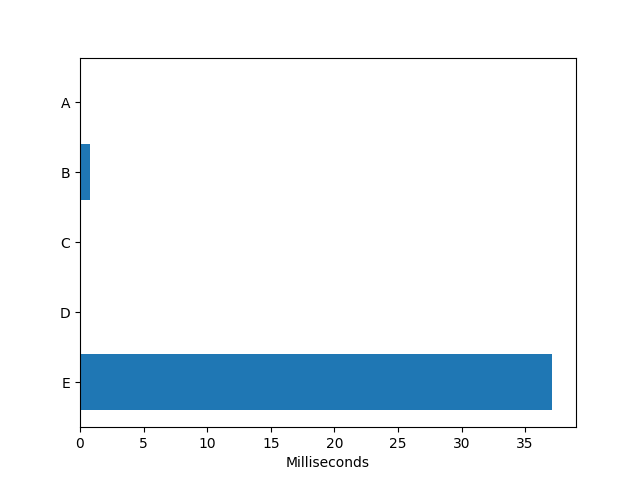
\includegraphics[width=\textwidth]{project-performance/graph_simple.png}
    \caption{Simple program}
  \end{subfigure}
  \begin{subfigure}[b]{0.46\textwidth}
    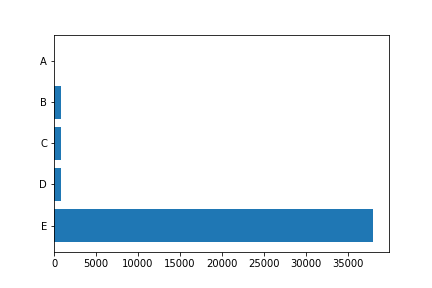
\includegraphics[width=\textwidth]{project-performance/graph_simple_c.png}
    \caption{Simple program (cumulative)}
  \end{subfigure}

  \begin{subfigure}[b]{0.46\textwidth}
    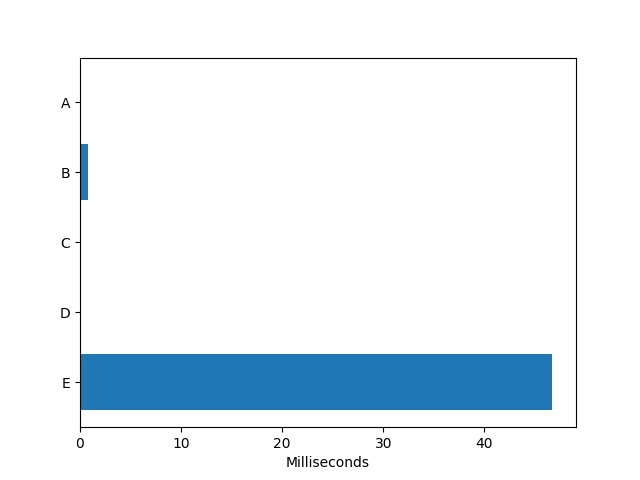
\includegraphics[width=\textwidth]{project-performance/graph_medium.png}
    \caption{Complex program}
  \end{subfigure}
  \begin{subfigure}[b]{0.46\textwidth}
    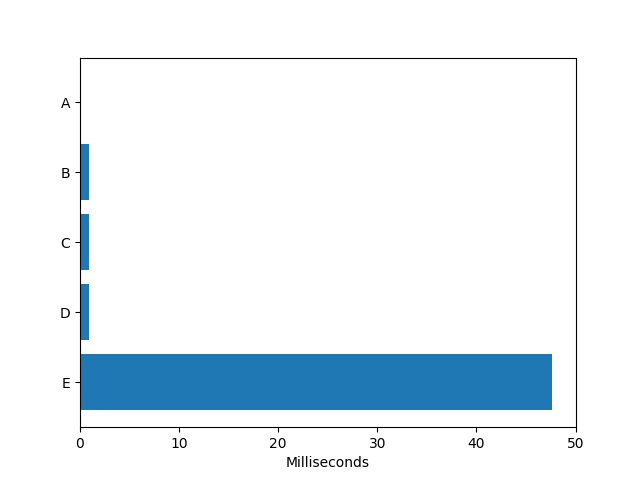
\includegraphics[width=\textwidth]{project-performance/graph_medium_c.png}
    \caption{Complex program (cumulative)}
  \end{subfigure}

  \caption{A graphic comparison of all the execution times, in $\mu s$.}
  \label{fig:perf-execution-times-comparison}
\end{figure}

\section{Conclusions and observations}

  \chapter{Conclusions}
  \section{WebAssembly and LSMs}

\textit{WebAssembly}, abbreviated to WASM, is a relatively new binary instruction format that
strives to bring security, speed, portability, and compactness to the Web
as a low-level alternative to JavaScript.
With the advent of the \textit{WebAssembly System Interface} (WASI),
this language can also be treated as a compilation target for languages such as C and Rust,
and can be executed directly on various operating systems
through the aid of runtimes, such as \textit{Wasmtime} and \textit{Wasmer}.

However, these runtimes' CLI interfaces do not provide a lot of user control
when dealing with the program's access rights to specific file system locations.
These interfaces can be extended by using pre-existing access control frameworks,
namely the \textit{Linux Security Modules}.
Specifically, two of these frameworks are taken into consideration - \textit{Landlock},
to provide unprivileged scoped access control, and \textit{eBPF}, a virtual
machine that can run sandboxed program in a privileged context.

\section{The developed project}

This thesis work deals with the development of a proof-of-concept WASM runtime that
provides the means to extend a WASM binary's access rights specifiable by the user.
The project is divided into three main phases.

Firstly, an analysis of the existing runtimes, \textit{Wasmtime} and \textit{Wasmer},
is required to understand how they behave in different situations and what
specific means they give to the user in order to restrict a WASM binary.
As highlighted in Section \ref{sec:introduction-wasi}, when using the default command line
interface, there is a lack of a fine granularity on what a program can do - for example,
the user cannot describe what a WASM binary is permitted to do on a preopened directory's files.

Secondly, the two LSMs in question, \textit{Landlock} and \textit{eBPF}, need to be studied and understood
so that they can be integrated with arbitrary code.
For this phase, having a mainstream Linux distro is not enough - these two LSMs have to be enabled
for them to be used by programs. This can be done either by manually compiling the kernel with the desired
flags enabled, or by using particular distros that have them enabled by default, such as Arch Linux.

Lastly, WASI libraries and the chosen LSMs have to be integrated in a new runtime, described in
Chapter \ref{chap:restricting-wasi}, able to run WASM binaries while simultaneously sandboxing them according to the user's choice.
When dealing with Landlock, the integration with a given program is provided by C libraries,
which can also be wrapped in the language of one's choice - for this project, this language is Rust,
in order to have a safer language that could still produce quite fast binaries.
On the other hand, eBPF has to be integrated externally, as the sandbox actions is done by
a server process, acting as a virtual machine.
Between the two, Landlock is definitely the easier one, both from a user's point of view,
regarding the available access control options, and from a developer's point of view, since
the existing libraries are quite straightforward to use. Moreover, its usage does not need the running program
to have root privileges.
The eBPF sandbox, although being more complex and requiring root privileges, is however
the more powerful one, allowing a great deal of fine tuning on multiple areas,
such as file system, network and inter-process communication.

Regarding performance, WASM is still not close to native speeds, and the usage of WASI libraries
brought a big overhead against the more traditional runtimes, as shown in the tests in Chapter \ref{chap:performance}.
However, LSMs themselves are not a hindrance on performance if considered in isolation.

\section{Possible improvements and future work}

The first problem that could be addressed is the performance of the WASI libraries.
In the testing runs, a very high percentage of the time is spent into loading and running the WASM module -
acting as a bottleneck, these libraries are thus the first and most effective point to improve.
This could be done either through optimisations in the original code, or through a more thorough
configuration of the library's execution capabilities.

Another possible improvement for the existing WASM runtimes could be the integration of \textit{Landlock}
if the development of a custom full-fledged access control framework turns out to be too great of
a challenge.
This could effectively bring a greater deal of control directly available to the user when
accessing the file system, while still being relatively simple to use.
However, Landlock is only available on Linux, and moreover it has to be enabled in the kernel.
This would pose two main problems:
\begin{enumerate}
  \item the runtime code would be less portable, since a custom version for Linux would have to be created, requiring
        the creation of more OS-specific code and making development more difficult;
  \item not all Linux users could use it, since enabling it can be a challenge that only more advanced users
        could be able and/or willing to face\footnote{This could be eased if Landlock were to be already enabled in most mainstream distros.}.
\end{enumerate}


  \nocite{*}
  \printbibliography[heading=bibintoc]
\end{document}